% !TeX spellcheck = en_US
\chapter{\iceact Simulation}\label{chap:iceact_sim}

This chapter will discuss the \geant simulation process. At first, simulations of the single optical components are studied in order to find appropriate parameters and settings for the whole optical system. Afterwards, an overall simulation is performed for the final goal of \iceact parameterization.

\section{Getting to Know the \iceact Optics}

In this section, the optical properties of \iceact are investigated in order to optimize their parameters. Possible uncertainties and aberration effects in the \iceact optics are examined by focusing on the single components: on the one hand, the effect of mounting a glass plate on top of the Fresnel lens is discussed. On the other hand, the approximation of the Winston cones by a tessellated structure might imply some aberrations or artifacts. 

\subsection{\enquote{Best} Wavelength}\label{sec:best_wvl}

Many of the \iceact telescope properties have (non-linear) wavelength dependencies (cf. section~\ref{sec:iceact:model:material}). Additionally, the Cherenkov spectrum is wavelength dependent as well (cf. figure~\ref{airshowers:cherenkovspectrum}). By implication, there has to be a wavelength $\lambda^\ast$ that \iceact is the most efficient. One can determine $\lambda^\ast$ by looking at the following limiting functions.

\begin{itemize}
	\item \textbf{The Cherenkov spectrum.} The data shown in figure~\ref{airshowers:cherenkovspectrum} (La Palma, \SI{2200}{\meter} a.s.l.) is chosen.
	\item \textbf{The internal transmission function of PMMA.} It is assumed that a photon has to pass approximately \SI{30}{\milli\meter} of PMMA to get to the SiPMs. Thus, the internal transmission function shown in figure~\ref{iceact:model:material:transmission} as blue dotted-dashed line has to be exponentiated by \num{10} to hold for this case.
	\item \textbf{The internal transmission function of borosilicate}, i.e. the material of the glass plate. The photons have to pass approximately \SI{2}{\milli\meter}. Exponentiation of a factor~$\frac{2}{3}$ of the orange dotted-dashed line in figure~\ref{iceact:model:material:transmission} leads to the desired function.
	\item \textbf{The photon detection efficiency (PDE) function of the SiPMs} interpolated for $V_\text{OV} = \SI{5}{\volt}$ (cf. orange curve in figure~\ref{sipm:pde}).
\end{itemize}

All of these functions are normalized, i.e. divided by their own maximum, and than multiplied which results in a new (relative) efficiency function. The maximum of this function again is the \enquote{best} wavelength found to be $\lambda^\ast = \SI{411}{\nano\meter}$. Figure~\ref{best_wvl} shows the procedure graphically. 

\begin{figure}[H]
	\centering
	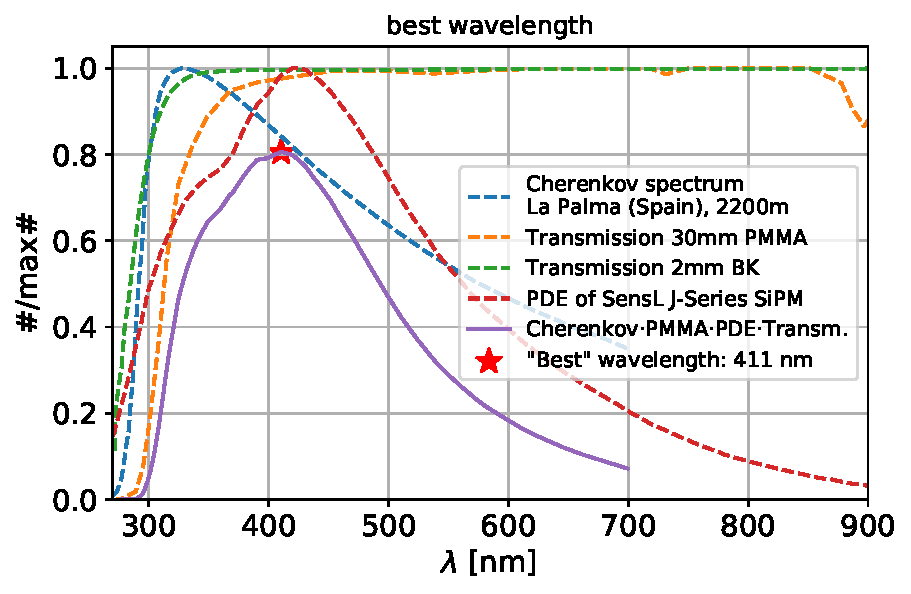
\includegraphics[width=0.7\textwidth]{best_wvl.pdf}
	\caption[\enquote{Best} wavelength]{\textbf{\enquote{Best} wavelength.} All limiting functions (Cherenkov spectrum, matrial transmission curves, and photon detection efficiency) are nomalized to each maximum and multiplied. The maximum of the product is defined to be the \enquote{best}, i.e. most efficient, wavelength $\lambda^\ast=\SI{411}{\nano\meter}$.}
	\label{best_wvl}
\end{figure}

\subsection{Focal Plane Shift}\label{sec:focalplaneshift}

So there is a most efficient wavelength for the \iceact telescope as shown in the last section~\ref{sec:best_wvl}. As stated in section~\ref{iceact:model:fresnellens} and in the ORAFOL data sheet~\cite{iceact:fresnellens:datasheet}, the focal distance of the Fresnel lens $z_f=\SI{502.1}{\milli\meter}$ is given for a certain wavelength $\lambda=\SI{546+-27.3}{\nano\meter}$. Thus, the focal distance at $\lambda^\ast=\SI{411}{\nano\meter}$ may be different which gives a possibility for potential improvement for the optical properties of \iceact. To investigate a shift of the focal plane, one has to define a quantity to optimize. In this simulation, the aberration radius $r_{90}$ is used for this purpose (cf. section~\ref{iceact:model:fresnellens}). A point spread function measurement of the Fresnel lens for monochromatic light with $\lambda=\SI{546}{\nano\meter}$ and different incidence angles $\theta$ is done in~\cite{famous:niggemann} by using ray tracing simulation. In this thesis, a PSF simulation is done as well but for wavelengths between $\SI{270}{\nano\meter}$ and $\SI{900}{\nano\meter}$ and vertical incidence $\theta=\SI{0}{\degree}$. The focal plane is fixed at the focal distance $z_f=\SI{502.1}{\milli\meter}$. In total, a vertical beam of \num{1e8} photons with uniformly density and uniformly distributed wavelengths in the interval given above is simulated. On the focal plane, the wavelength $\lambda_\text{hit}$, position $(x_\text{hit},y_\text{hit}))$, and angle $(\theta_\text{hit},\phi_\text{hit})$ of the detected photons are registered. The goal is to measure the minimal aberration radius at the suggested focal distance $z_f=\SI{502.1}{\milli\meter}$ and a possible focal plane shift in order to minimize the aberration radius for $\lambda^\ast=\SI{411}{\nano\meter}$.\\

For the first measurement, the aberration radius is evaluated by calculating the \SI{90}{\percent}-quantile of the distances $r_\text{hit}$ between the hit position and the optical axis\footnote{Normally, this is the centroid rather than the optical axis but in the case of parallel light, the centroid is assumed to be at $(x,y) = (0,0)$.} given by
\begin{align}
	r_\text{hit} = \sqrt{\left(x_\text{hit}-x_\text{centroid}\right)^2+\left(y_\text{hit}-y_\text{centroid}\right)^2} \overset{(x,y)_\text{centroid}=(0,0)}{=}\sqrt{x_\text{hit}^2+y_\text{hit}^2}\,.
\end{align}
By doing this for small wavelength ranges, one gets a wavelength-dependent aberration radius $r_{90}(\lambda)$ on the focal plane. As a result, a minimal aberration radius of \SI{1.78}{\milli\meter} is reached at a wavelength of \SI{403}{\nano\meter}. Figure~\ref{psf_at_focal_plane} shows $r_{90}(\lambda)$.\\

\begin{figure}[H]
	\centering
	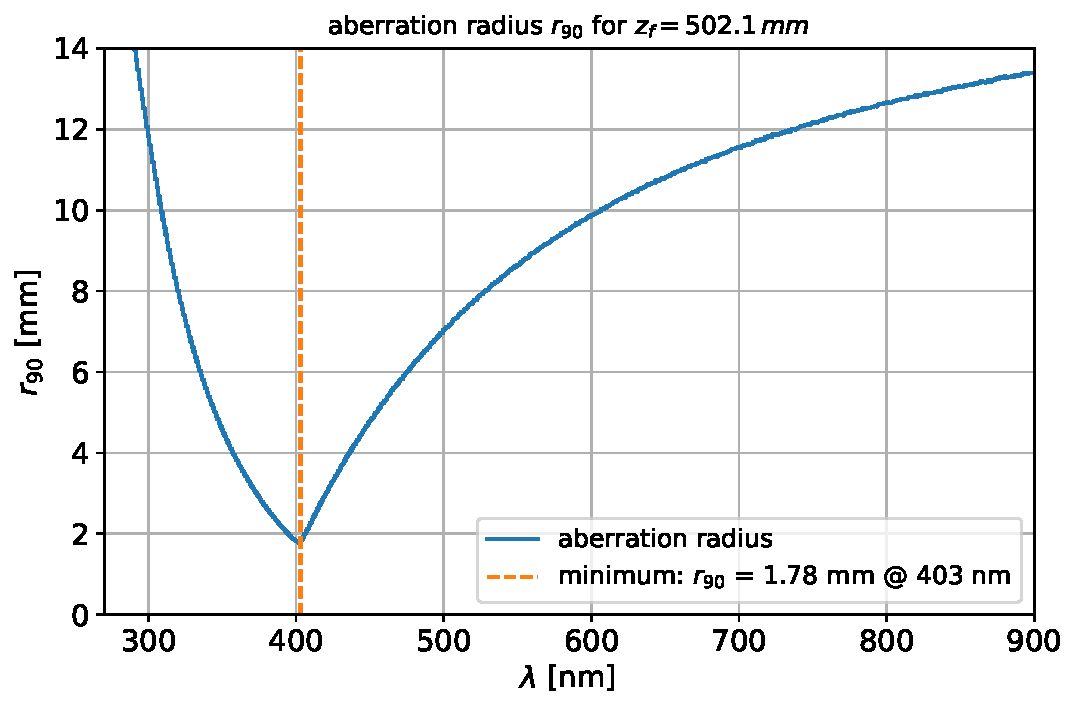
\includegraphics[width=0.8\textwidth]{focalplaneshift/psf_r90.pdf}
	\caption[Aberration radius on the focal plane]{\textbf{Aberration radius on the focal plane.} $r_{90}$ is calculated for vertical light as a function of the wavelength. The focal distance is fixed to $z_f=\SI{502.1}{\milli\meter}$. The minimal aberration radius of \SI{1.78}{\milli\meter} is reached at a wavelength of \SI{403}{\nano\meter}.}
	\label{psf_at_focal_plane}
\end{figure}

For the focal plane shift, one considers a small wavelength range and again calculates the aberration radius. Since the incidence angles on the focal plane are known, one can calculate the point of incidence for a hypothetical focal plane at a position of $z_f+\Delta z$, where $\Delta z$ is the focal plane shift. A trigonometrical approach gives
\begin{align}
	r_\text{hit}(\Delta z) = \sqrt{\left(x_\text{hit}-\Delta z\tan\theta_\text{hit}\cos\phi_\text{hit}\right)^2 + \left(y_\text{hit}-\Delta z\tan\theta_\text{hit}\sin\phi_\text{hit}\right)^2}\,.
\end{align}
Thus, the aberration radius can be calculated for each focal plane shift $\Delta z$ and wavelength $\lambda$. Than, an optimal focal plane shift can be found by minimizing the aberration radius. Figure~\ref{focalplaneshift} shows this calculation for different wavelengths by evaluation the beam \enquote{caustic}\footnote{In this context, caustic means the photon density distribution along the optical axis. Usually in beam optics, a caustic just describes the envelope of the beam.} for different focal plane shifts. One can clearly see that the focal length increases with wavelength. Additionally, figure~\ref{focalplaneshift_zoomout} shows a zoomed-out version of figure~\ref{focalplaneshift_bestwvl}. In particular for the most efficient wavelength $\lambda^\ast=\SI{411}{\nano\meter}$, a resulting marginal focal plane shift of $\Delta z=\SI{1.25}{\milli\meter}$ shows, that the standard focal distance is already quite good for \iceact. Nevertheless, the focal plane shift is considered in the final parameterization simulation.

\begin{figure}[H]
	\centering
	\begin{subfigure}[t]{0.48\textwidth}
		\centering
		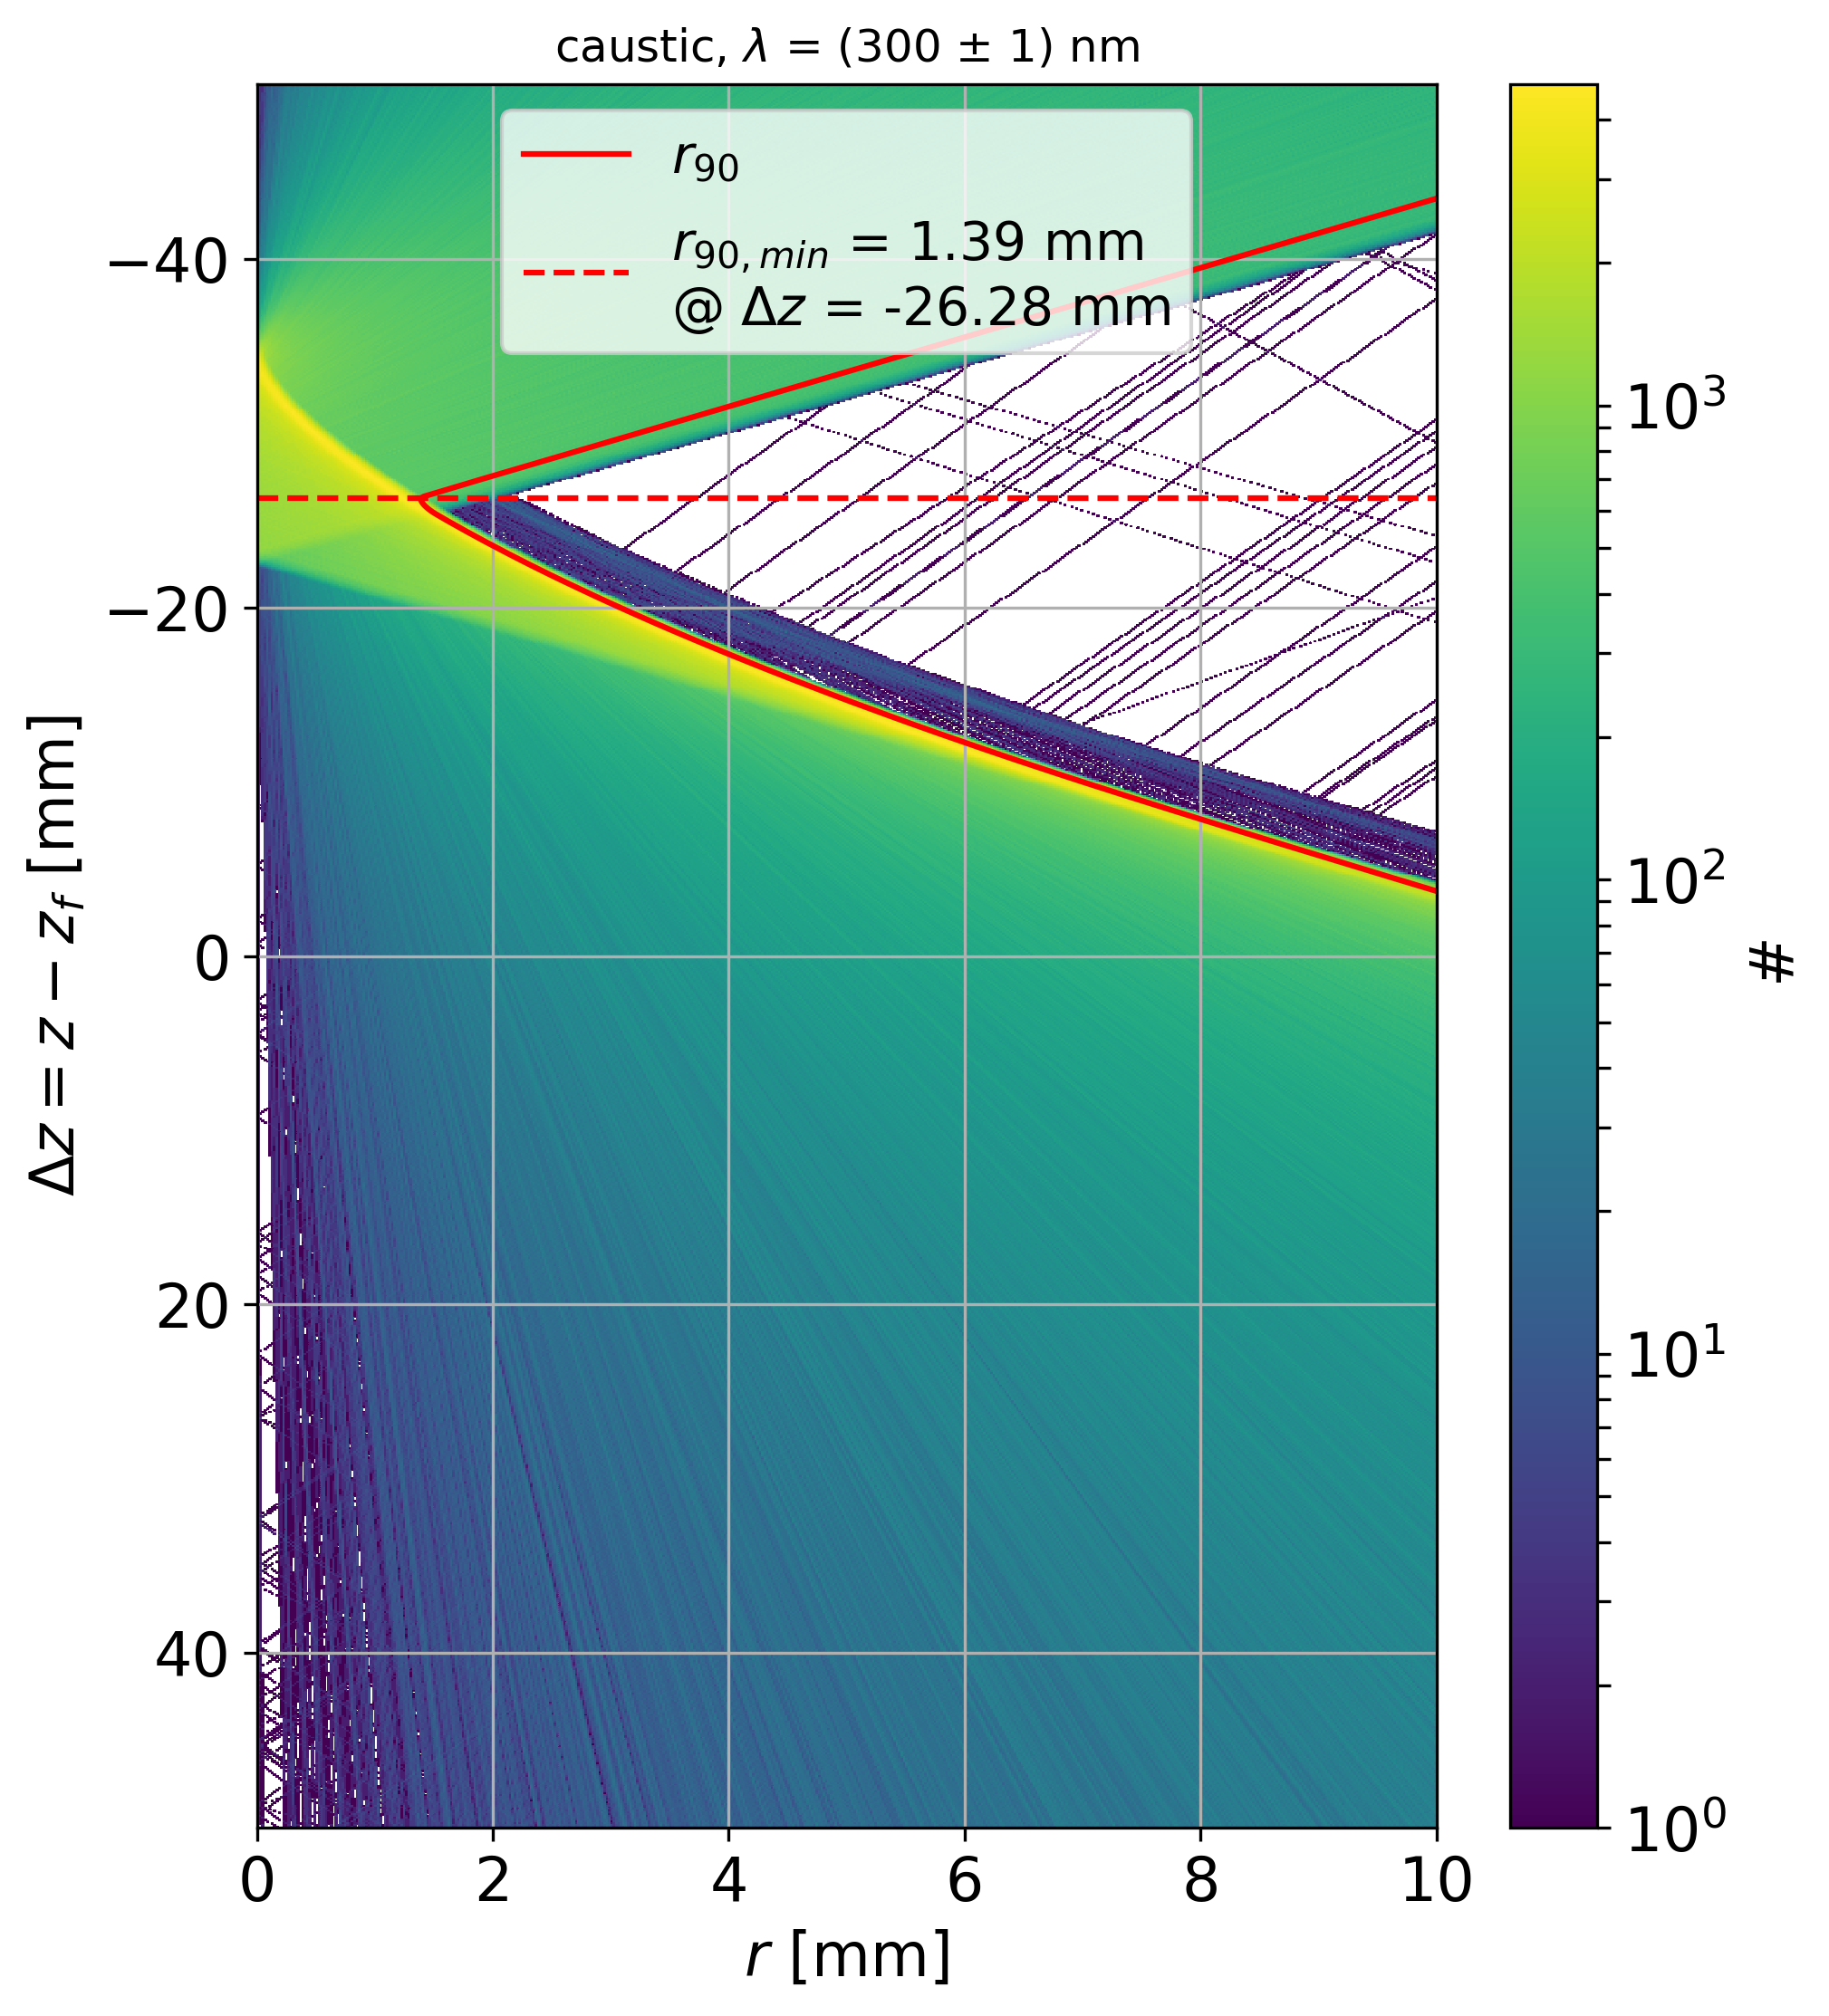
\includegraphics[width=\textwidth]{focalplaneshift/caustic_300nm.png}
		\subcaption{$\lambda=\SI{300+-1}{\nano\meter}$}
	\end{subfigure}
	\hfill
	\begin{subfigure}[t]{0.48\textwidth}
		\centering
		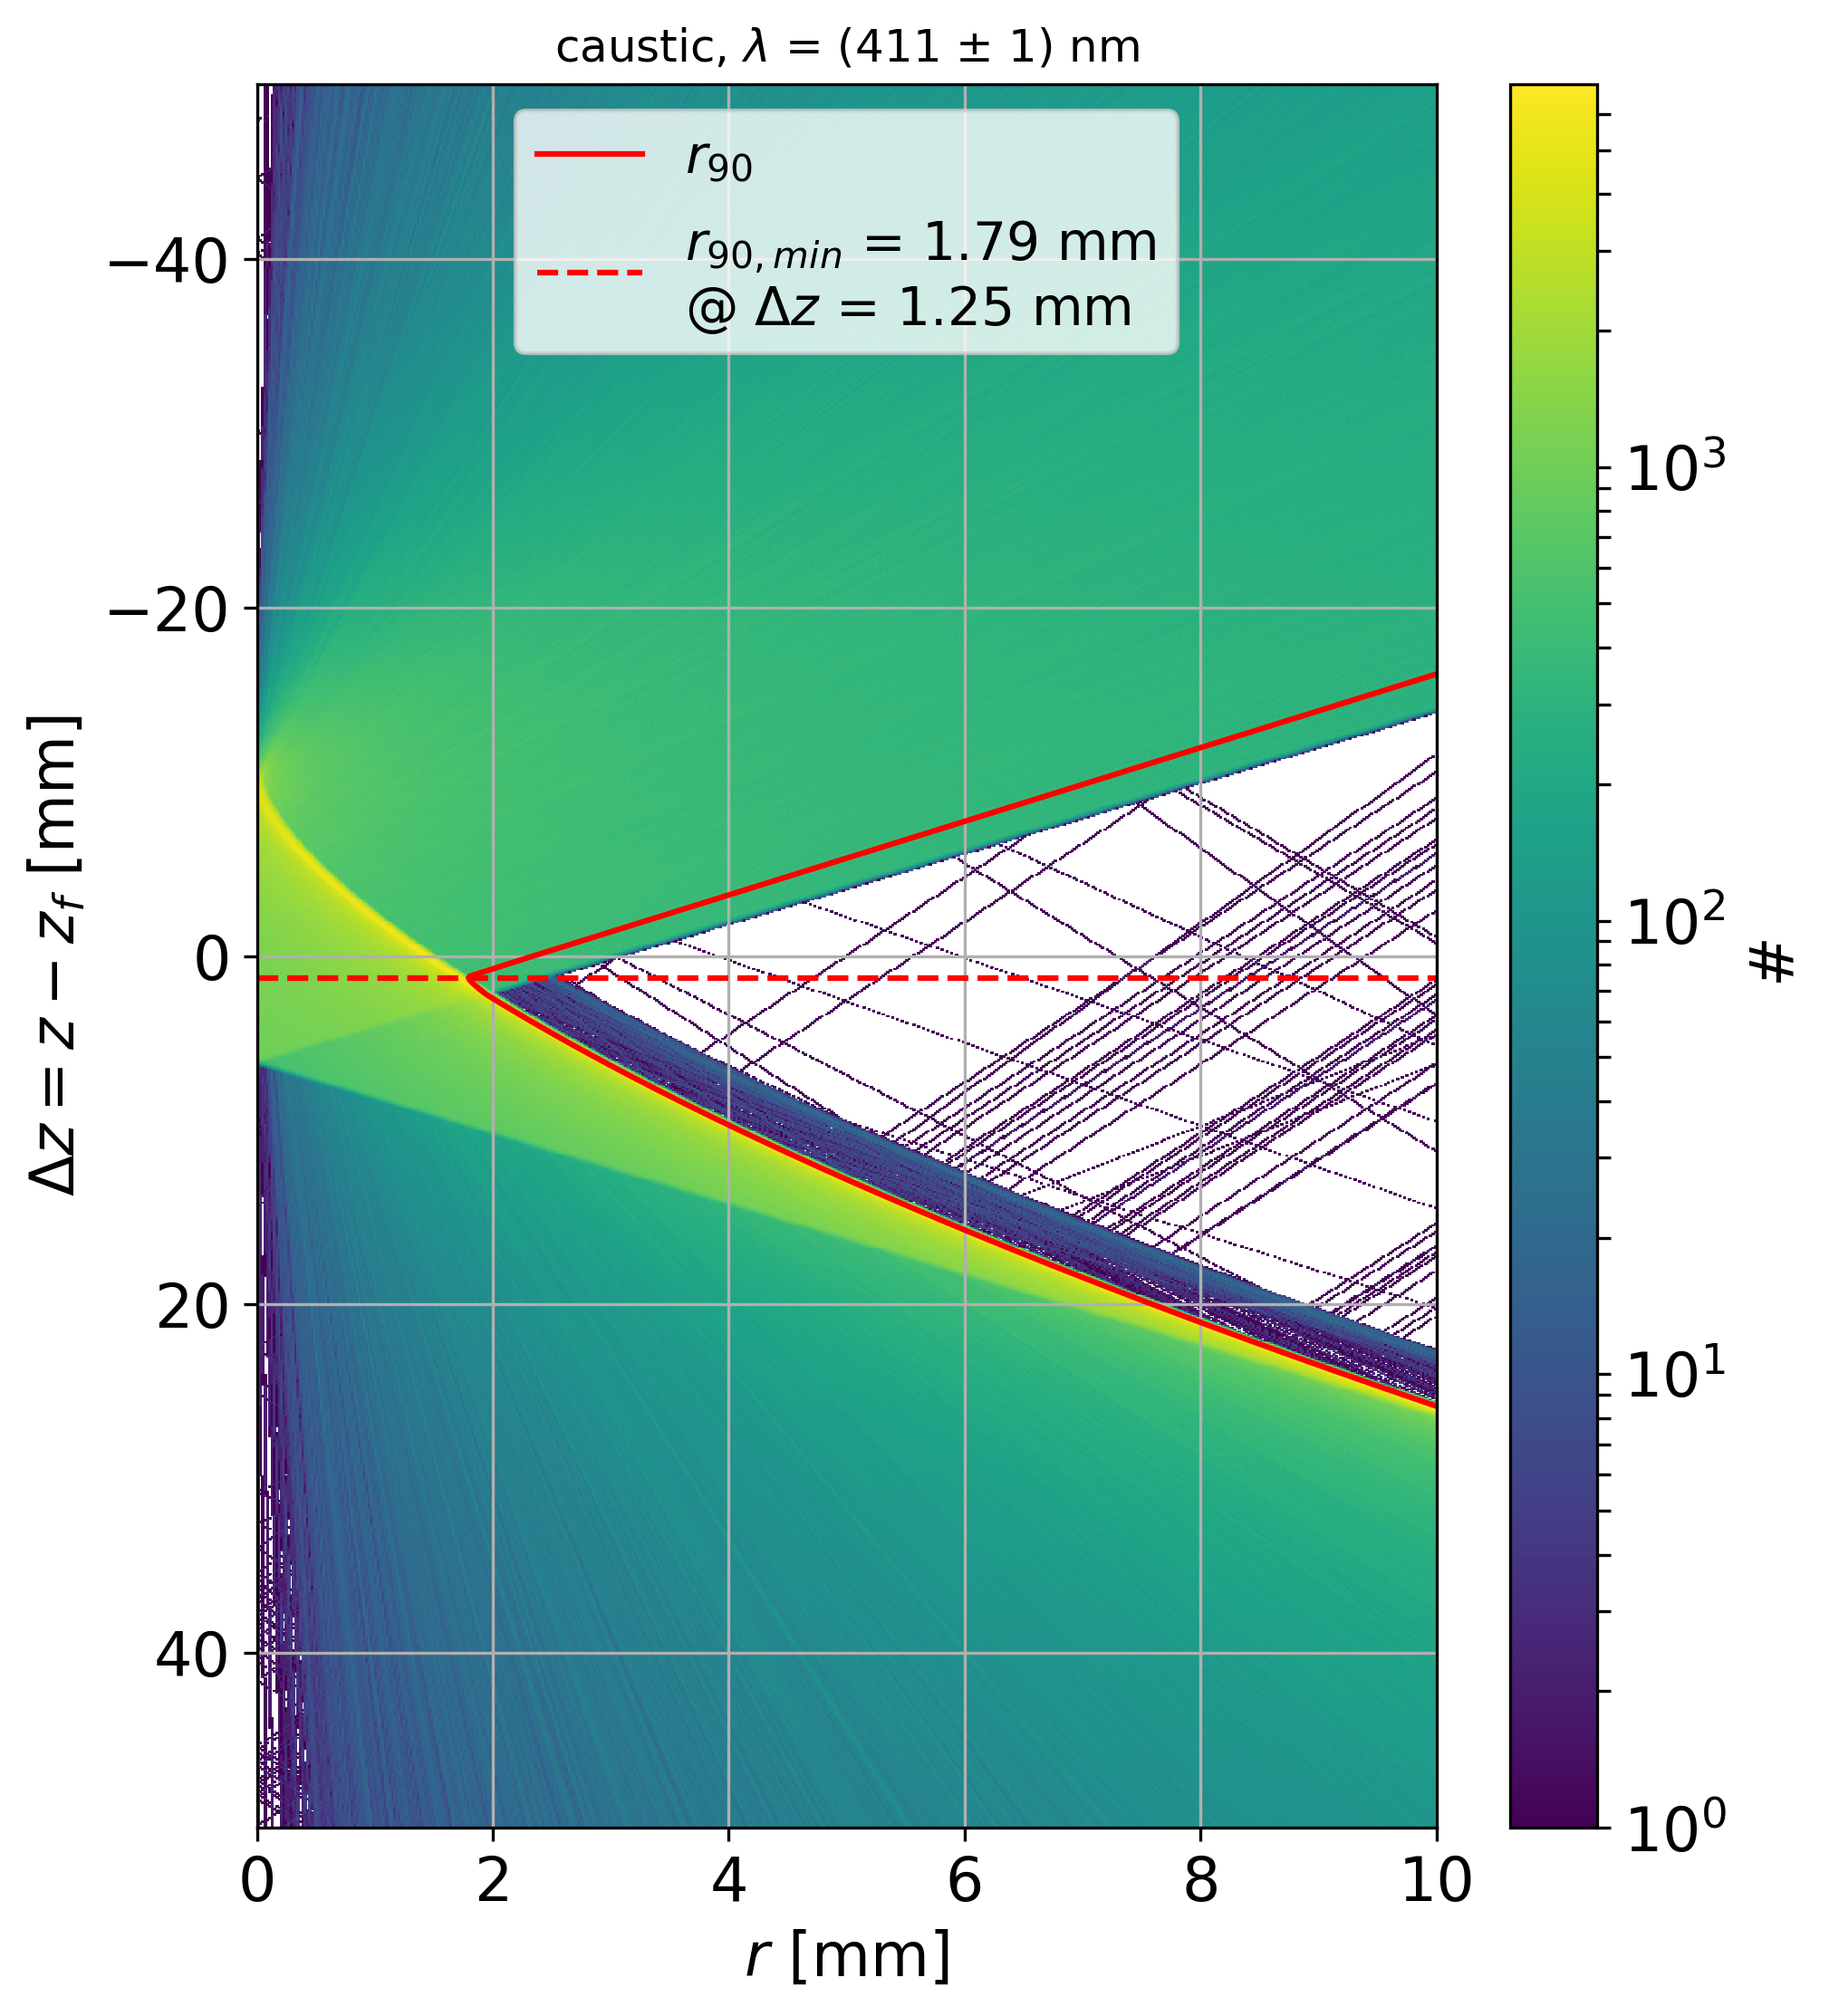
\includegraphics[width=\textwidth]{focalplaneshift/caustic_411nm.png}
		\subcaption{$\lambda^\ast=\SI{411+-1}{\nano\meter}$}
		\label{focalplaneshift_bestwvl}
	\end{subfigure}
	\hfill
	\begin{subfigure}[t]{0.48\textwidth}
		\centering
		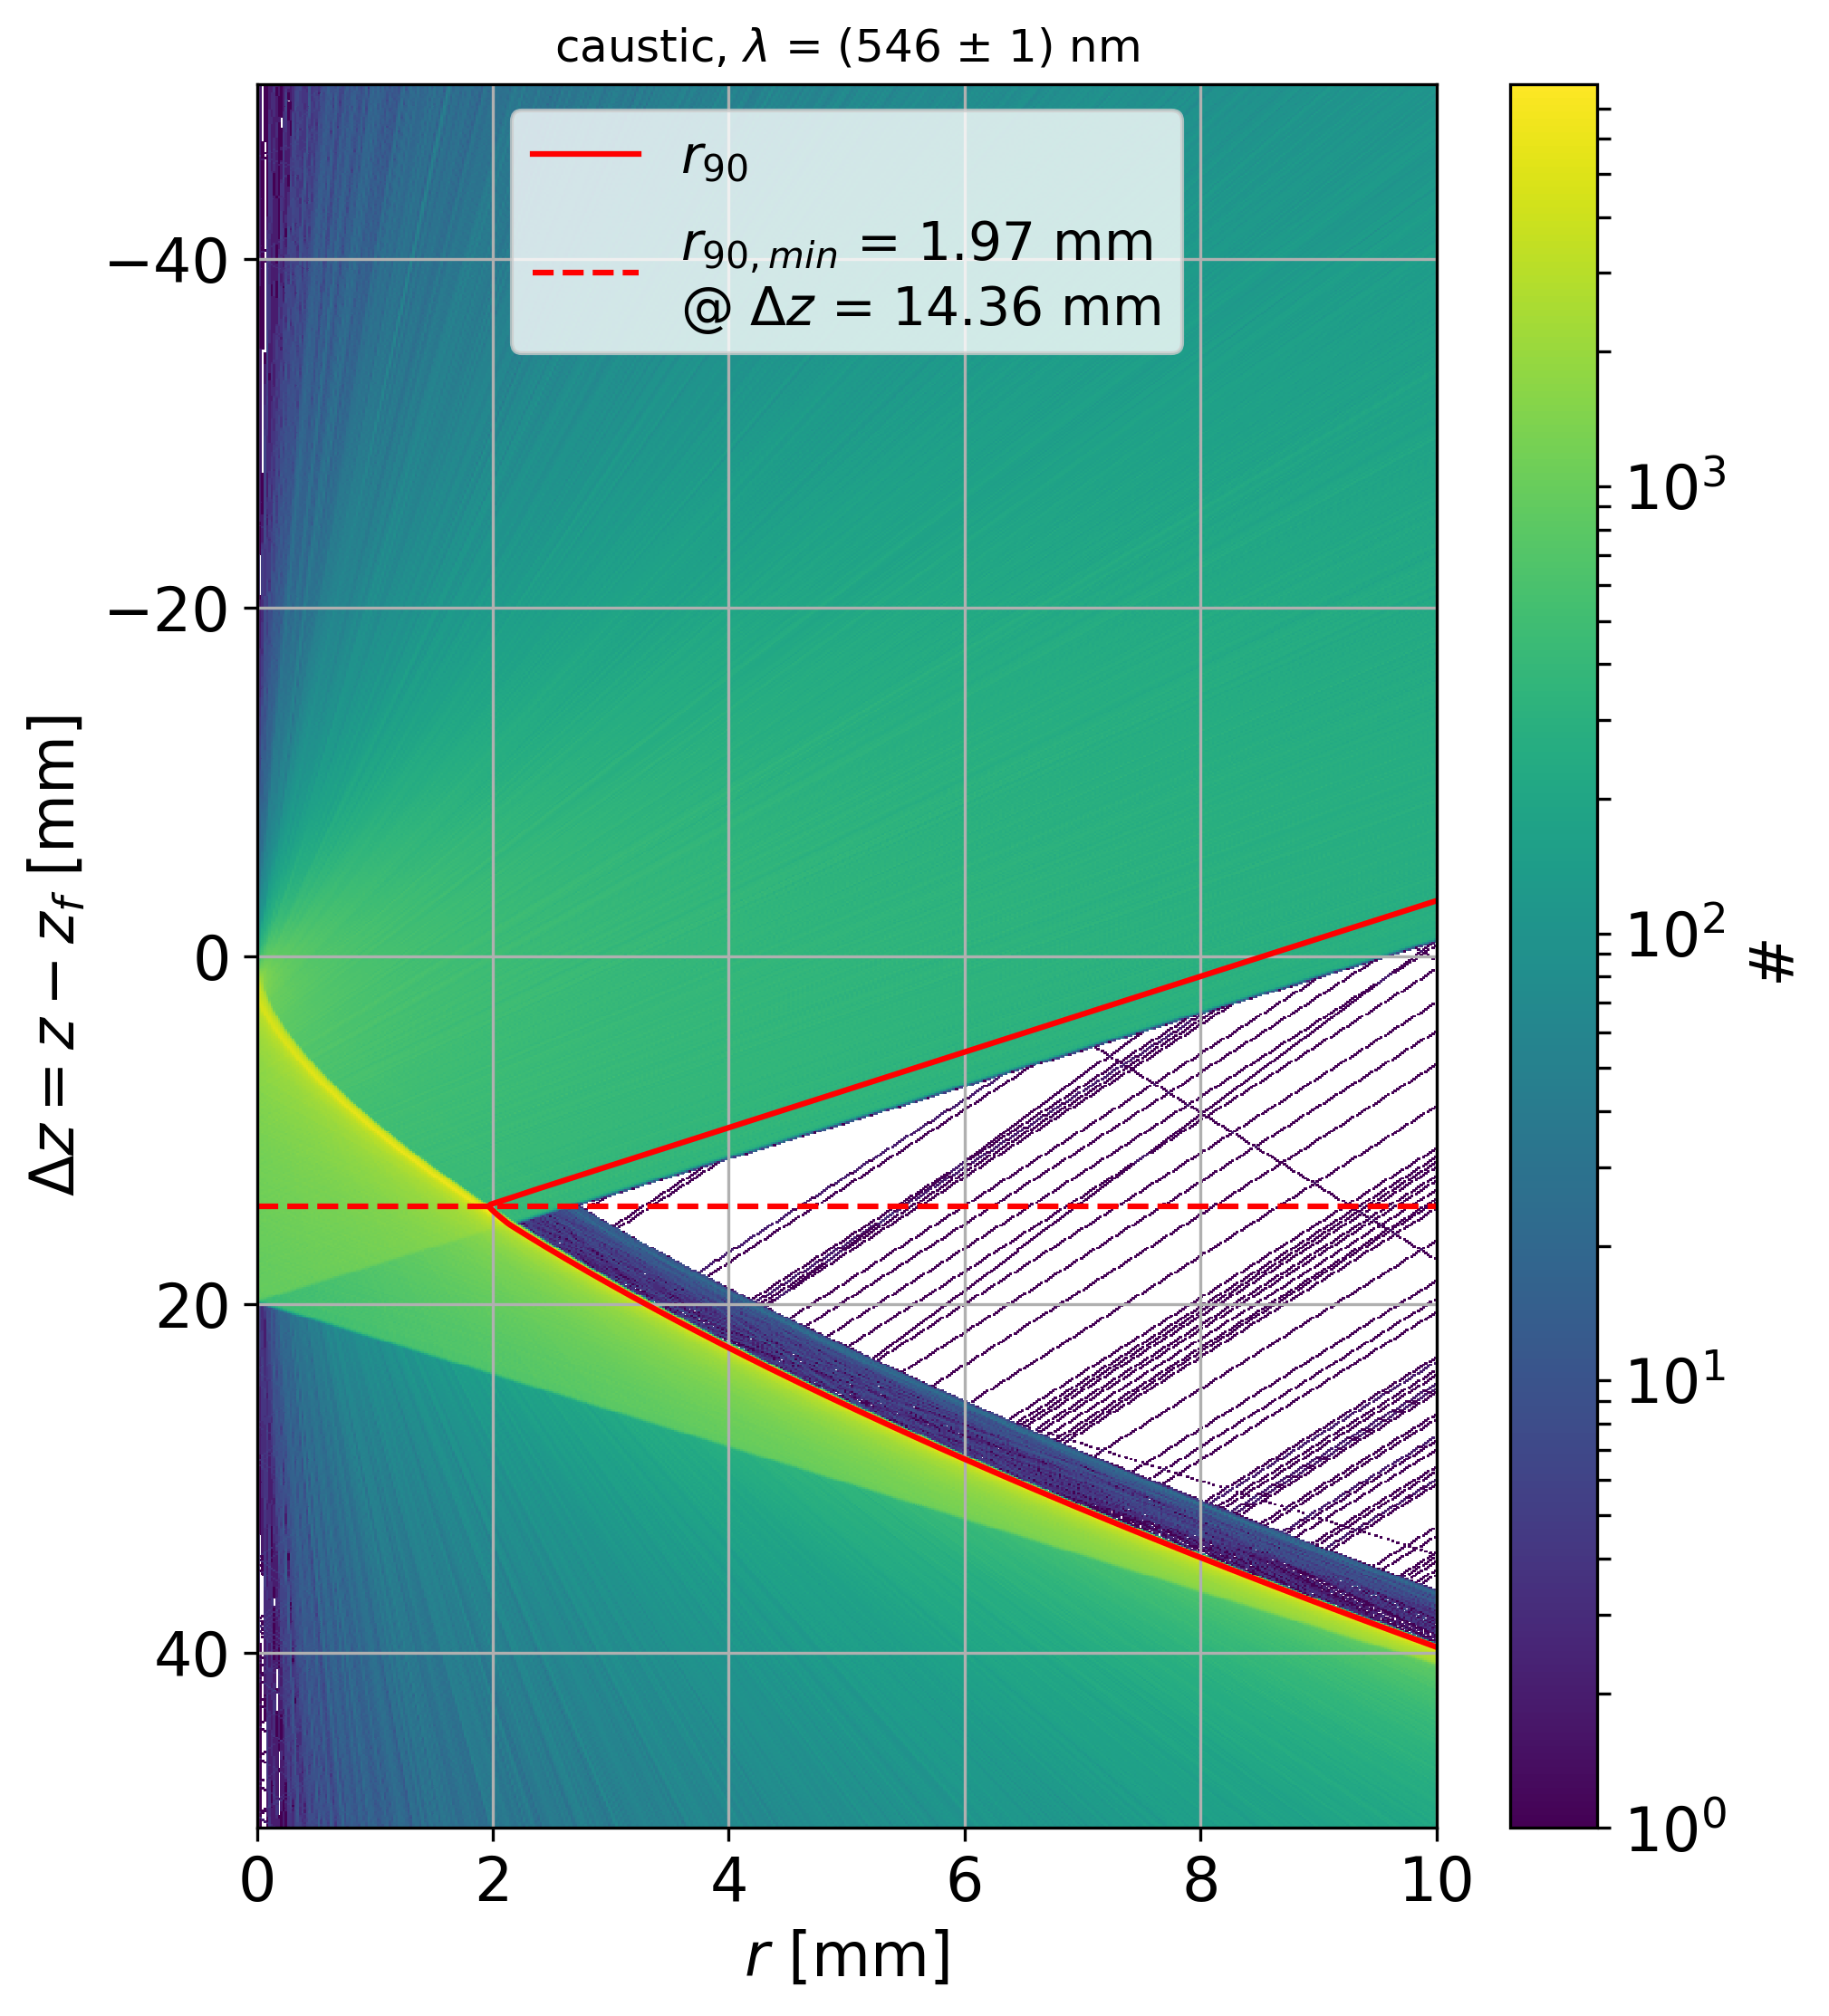
\includegraphics[width=\textwidth]{focalplaneshift/caustic_546nm.png}
		\subcaption{$\lambda=\SI{546+-1}{\nano\meter}$}
		\label{focalplaneshift_famouswvl}
	\end{subfigure}
	\hfill
	\begin{subfigure}[t]{0.48\textwidth}
		\centering
		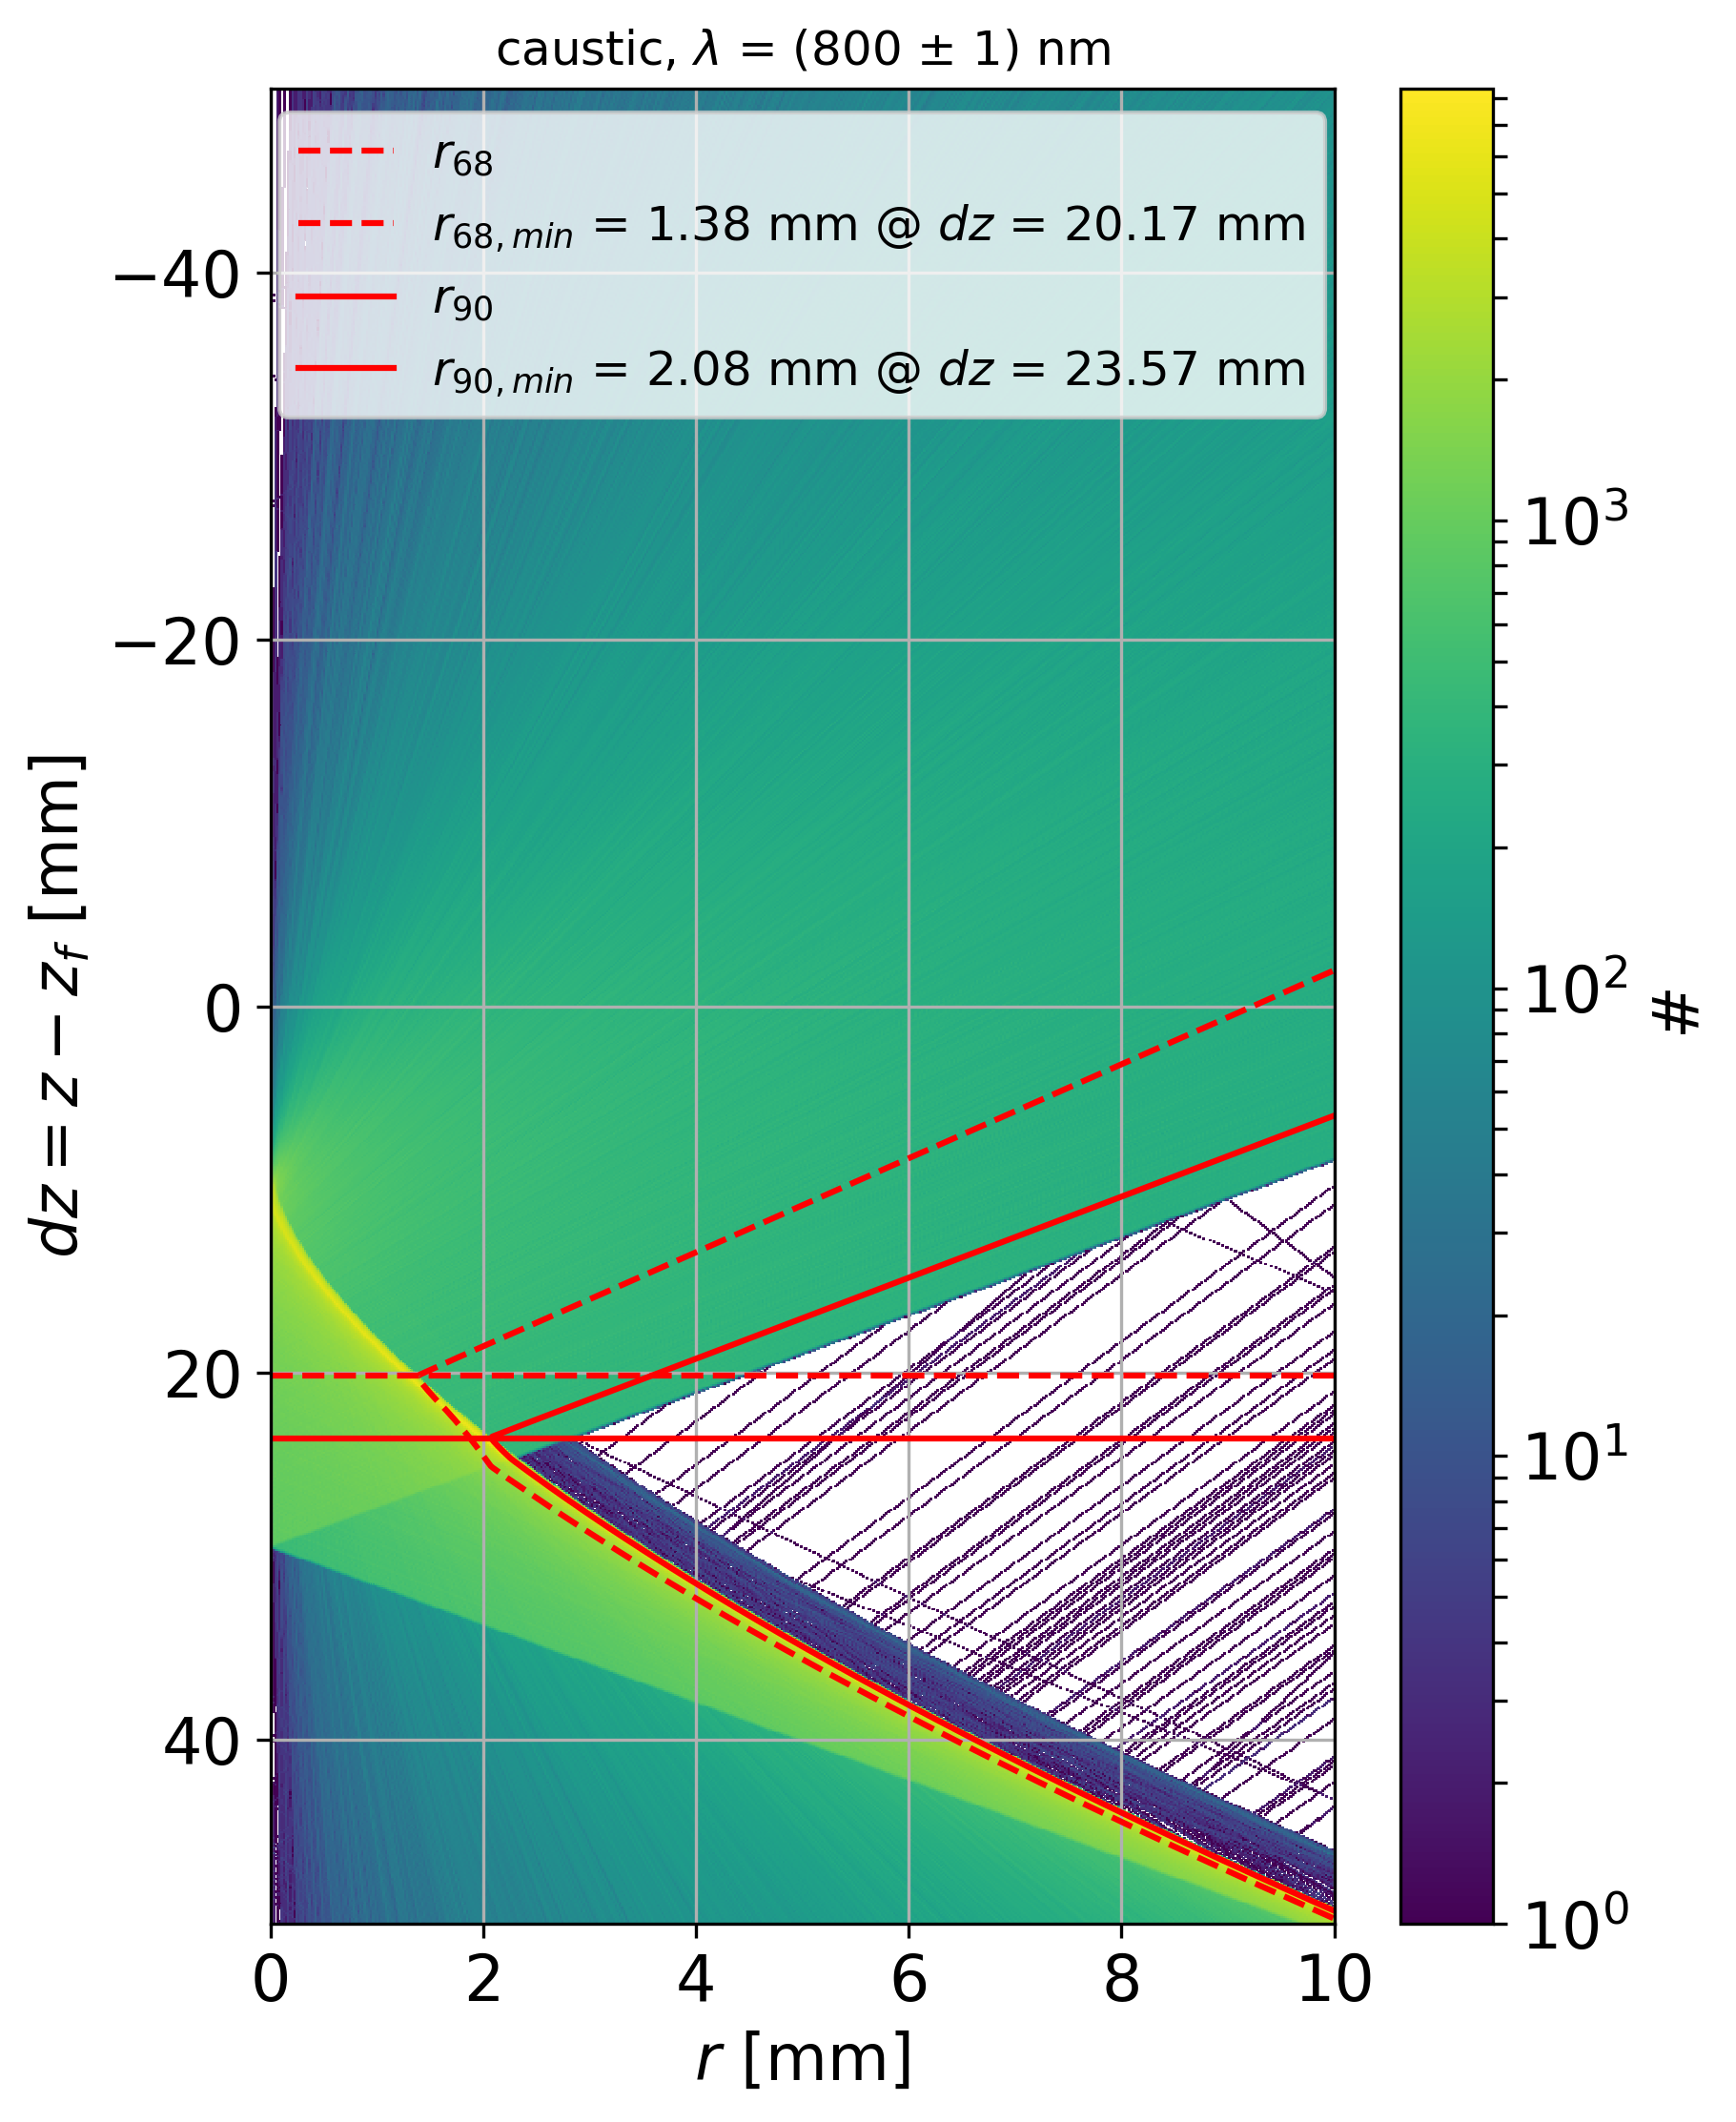
\includegraphics[width=\textwidth]{focalplaneshift/caustic_800nm.png}
		\subcaption{$\lambda=\SI{800+-1}{\nano\meter}$}
	\end{subfigure}
	\caption[\enquote{Caustic} histograms for the focal plane shift]{\textbf{\enquote{Caustic} histograms for the focal plane shift.} For focal plane shifts~$\Delta z$ between $\SI{-50}{\milli\meter}$ and $\SI{50}{\milli\meter}$, the incident positions of simulated photons are histrogramized by calculating their distance from the optical axis $r_\text{hit}(\Delta z)$. This results in a photon density plot called \enquote{caustic}. A focal plane shift of $\Delta z = 0$ is equivalent to the \enquote{standard} focal distance $z_f=\SI{502.1}{\milli\meter}$. A positive $\Delta z$ connotes a shift away from the lens. Thus, the lens is located on top of the shown plots. The calculation is done for different wavelengths, especially for the \enquote{best} wavelength in (\subref{focalplaneshift_bestwvl}) and for the wavelength which the focal distance is set for in (\subref{focalplaneshift_famouswvl}). The red line shows the aberration radius $r_{90}(\Delta z)$ and the focal plane shift where its minimum is reached marked by the red dashed line.}
	\label{focalplaneshift}
\end{figure}

\begin{figure}[H]
	\centering
	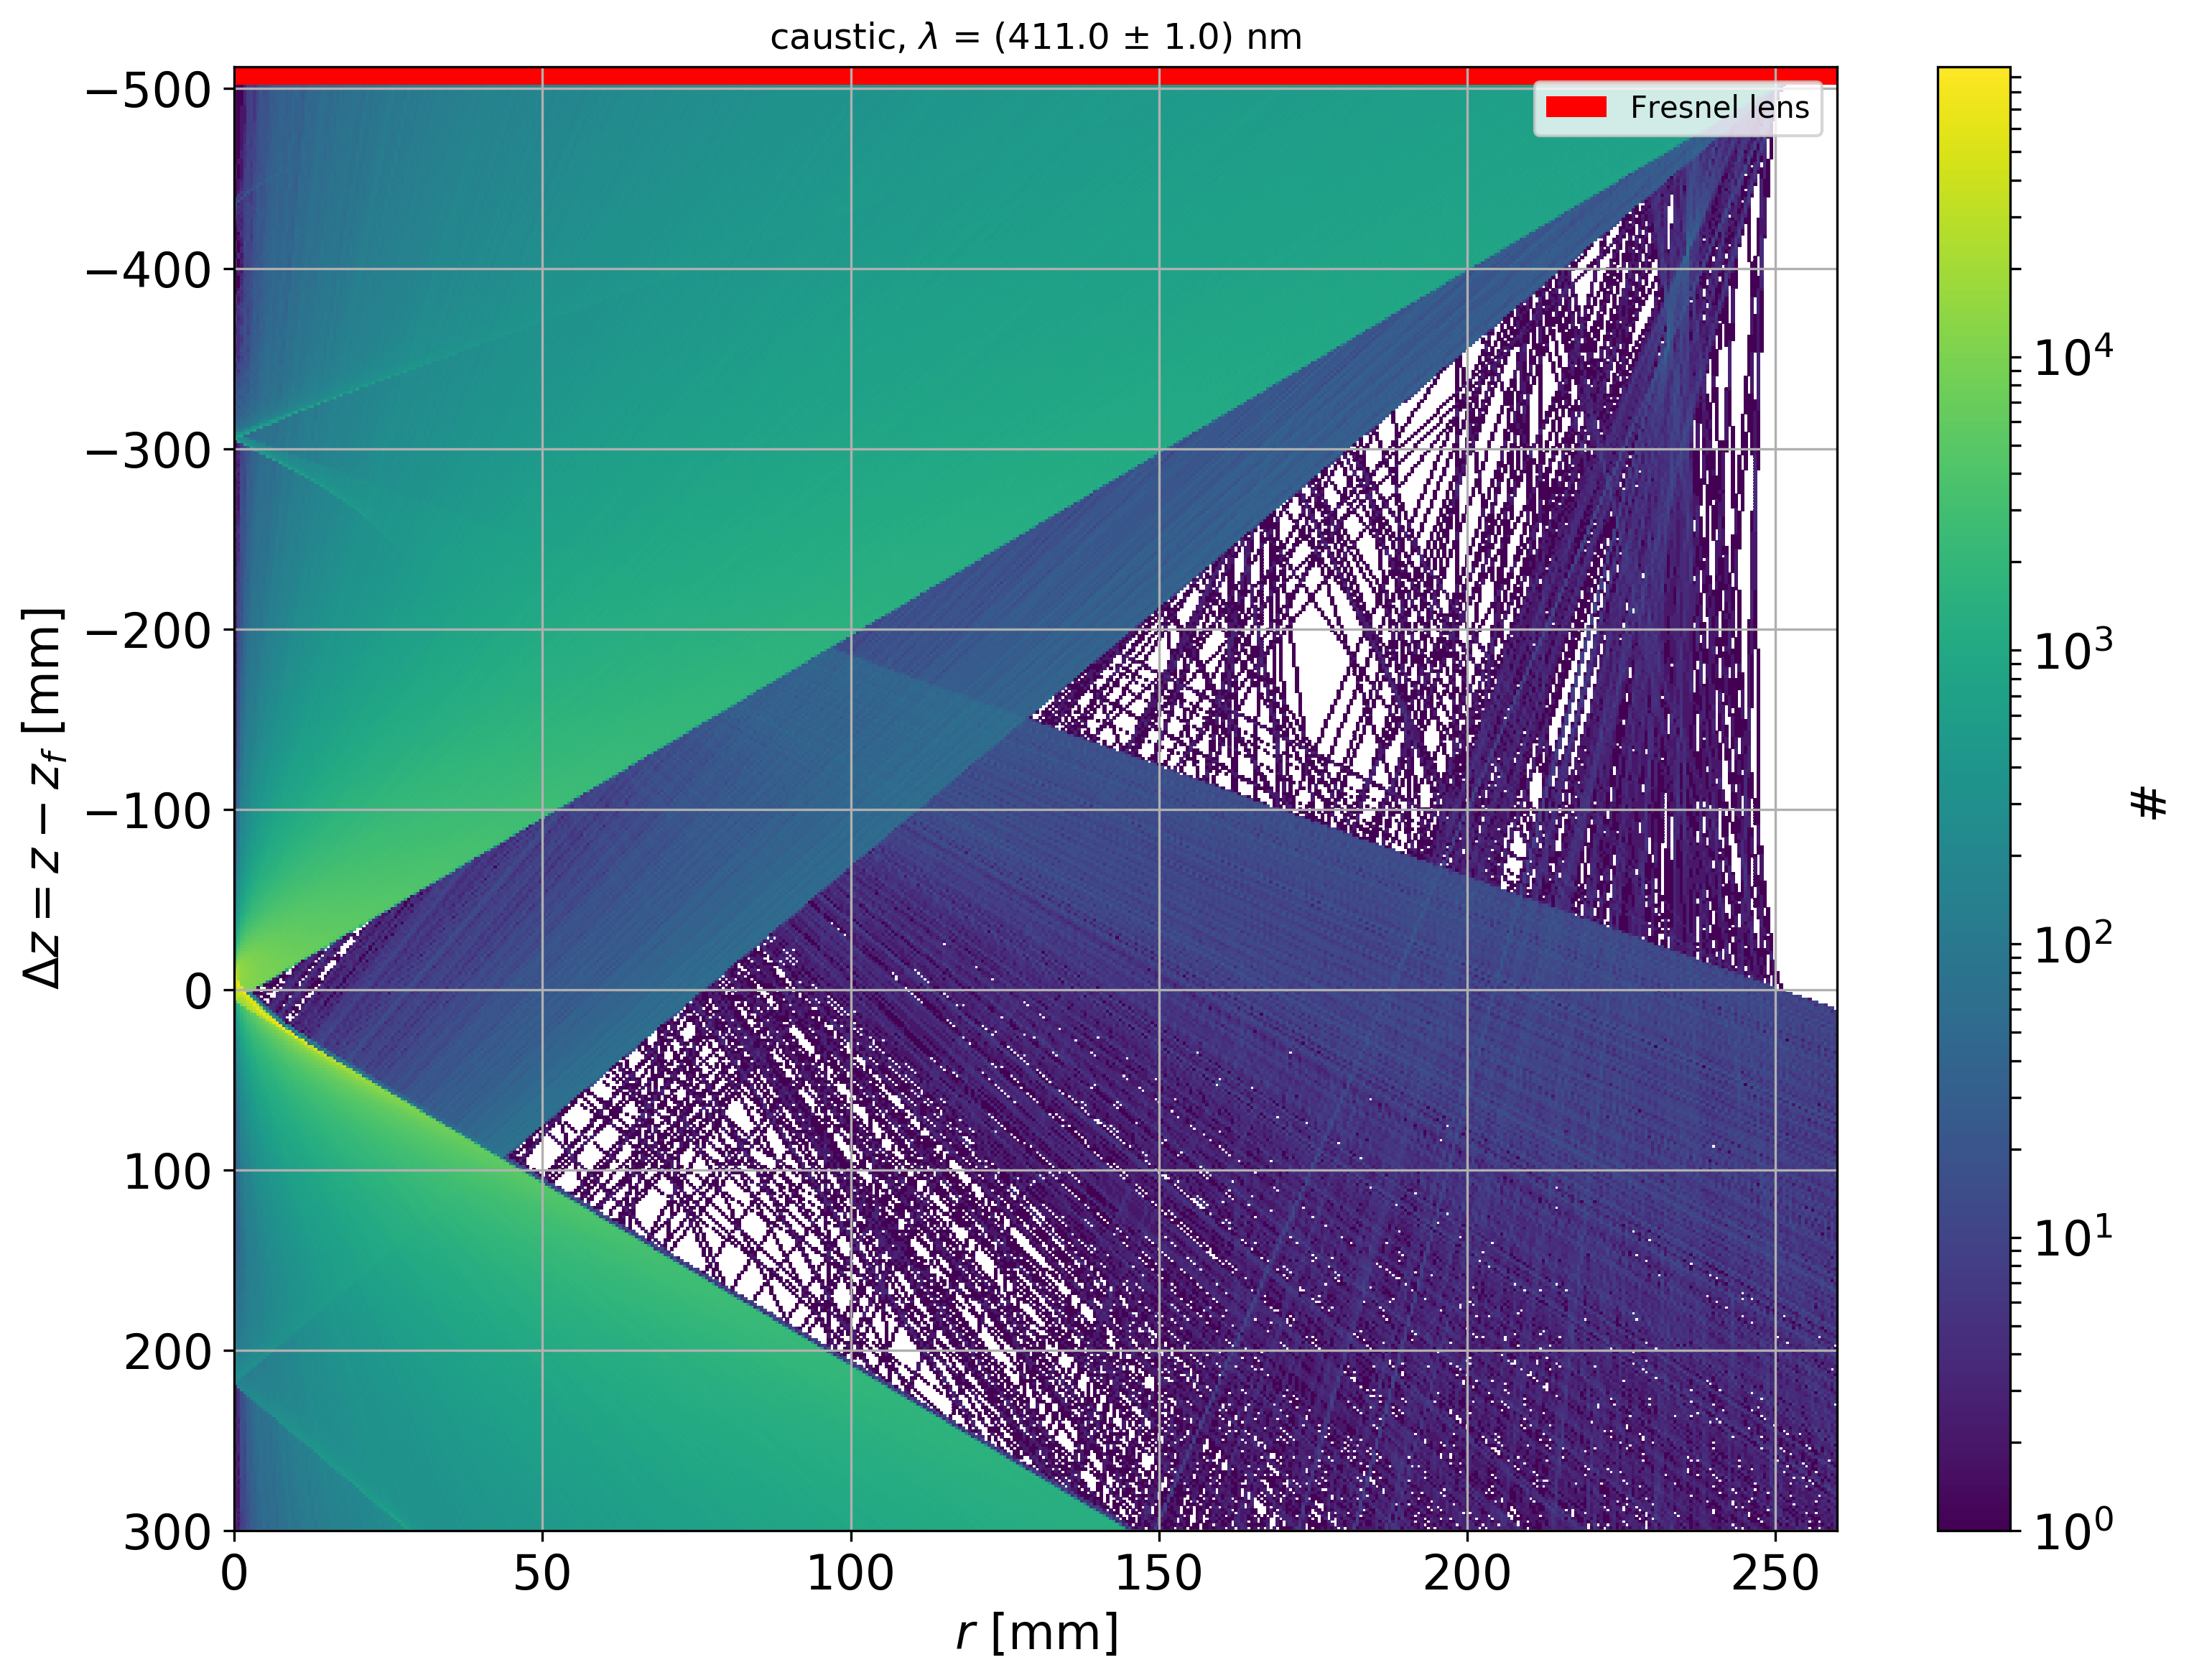
\includegraphics[width=0.8\textwidth]{focalplaneshift/caustic_411nm_zoomout.png}
	\caption[Zoomed-out caustic histogram]{\textbf{Zoomed-out caustic histogram.} The plot shows a zoomed-out version of figure~\ref{focalplaneshift_bestwvl}. The red band on the top denotes the location of the Fresnel lens. Besides a major focal spot at $\Delta z\approx\SI{0}{\milli\meter}$, one can see two minor ones at $\Delta z\approx\SI{-300}{\milli\meter}$ and $\Delta z\approx\SI{220}{\milli\meter}$ which come from the \enquote{false} refractions mentioned in section~\ref{iceact:model:fresnellens}.}
	\label{focalplaneshift_zoomout}
\end{figure}

\subsection{Winston Cone Meshing}\label{sec:wico_meshing}

As already brought up in section~\ref{sec:winstoncones:impl}, the \textit{mesh size} $m$ -- i.e. the maximum edge length of the meshed Winston cone model -- has to be chosen as a compromise between imaging quality and computational effort. For the \iceact parameterization, especially the light collection capability of the Winston cone is necessary rather than its actual imaging quality. Nevertheless, the meshing is chosen to have a sufficiently high level of detail to avoid coarse imaging artifacts. Figure~\ref{wico:theta0_image} shows very obviously that the higher the mesh size the coarser the artifacts get. 

\begin{figure}[H]
	\centering
	\begin{subfigure}[t]{0.495\textwidth}
		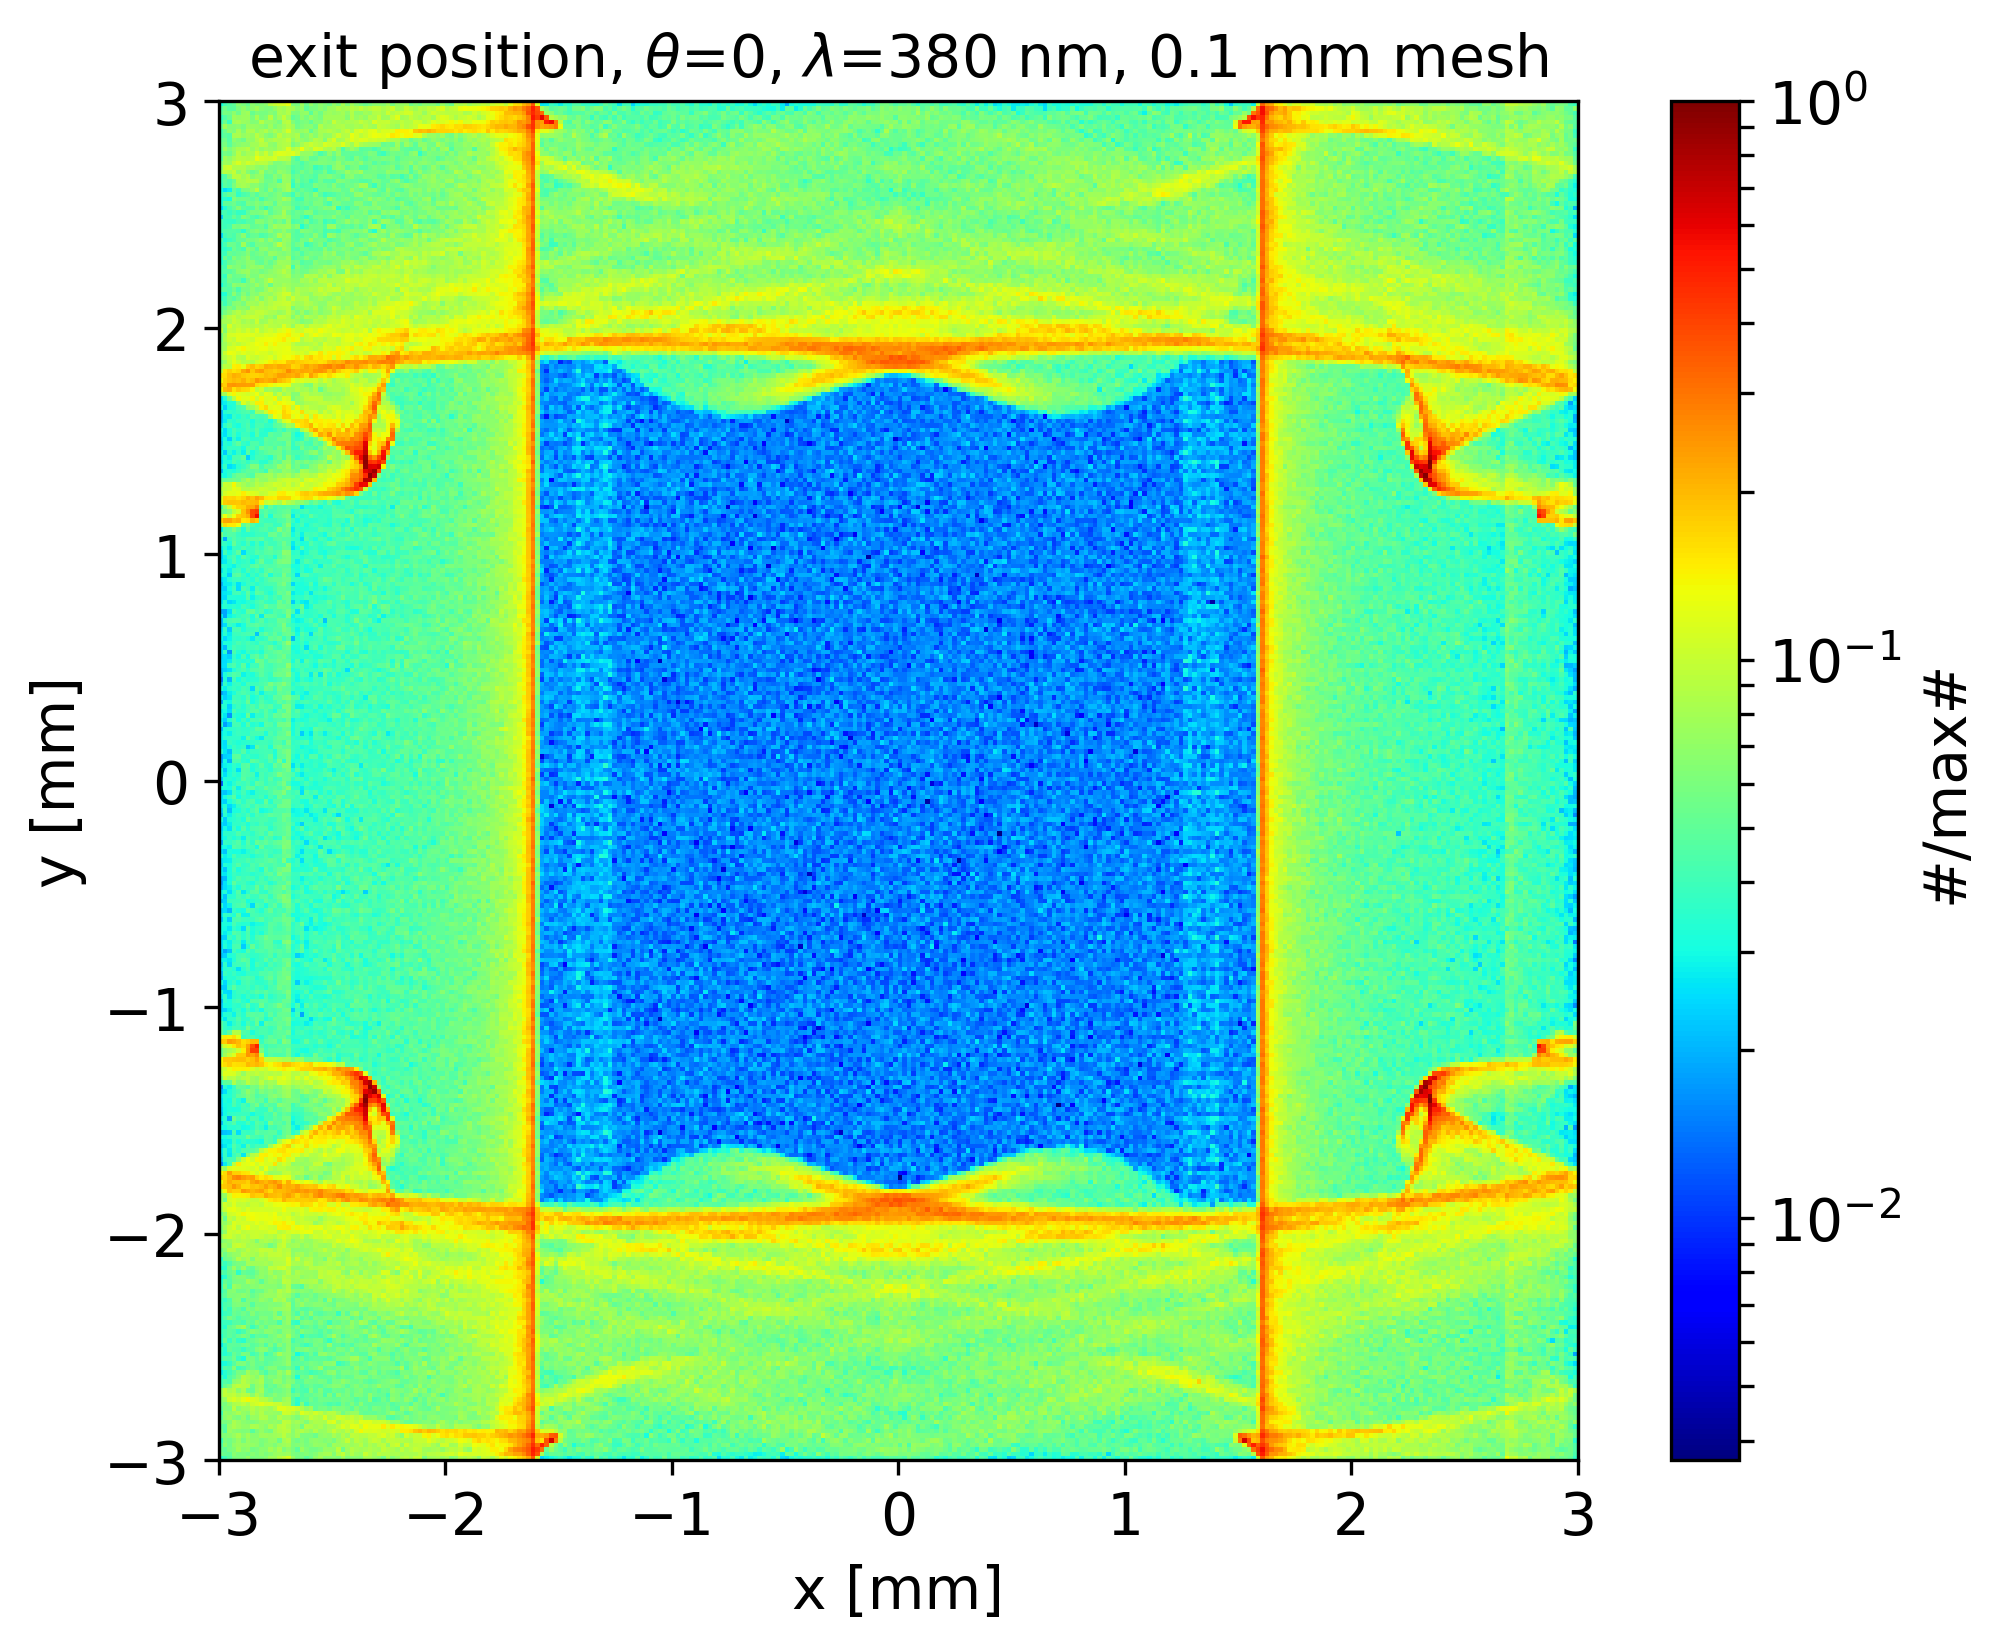
\includegraphics[width=\textwidth]{wico-theta0/hist_theta0_380nm-0.1mmMesh_log.png}
		\subcaption{$m=\SI{0.1}{\milli\meter}$.}
	\end{subfigure}
	\hfill
	\begin{subfigure}[t]{0.495\textwidth}
		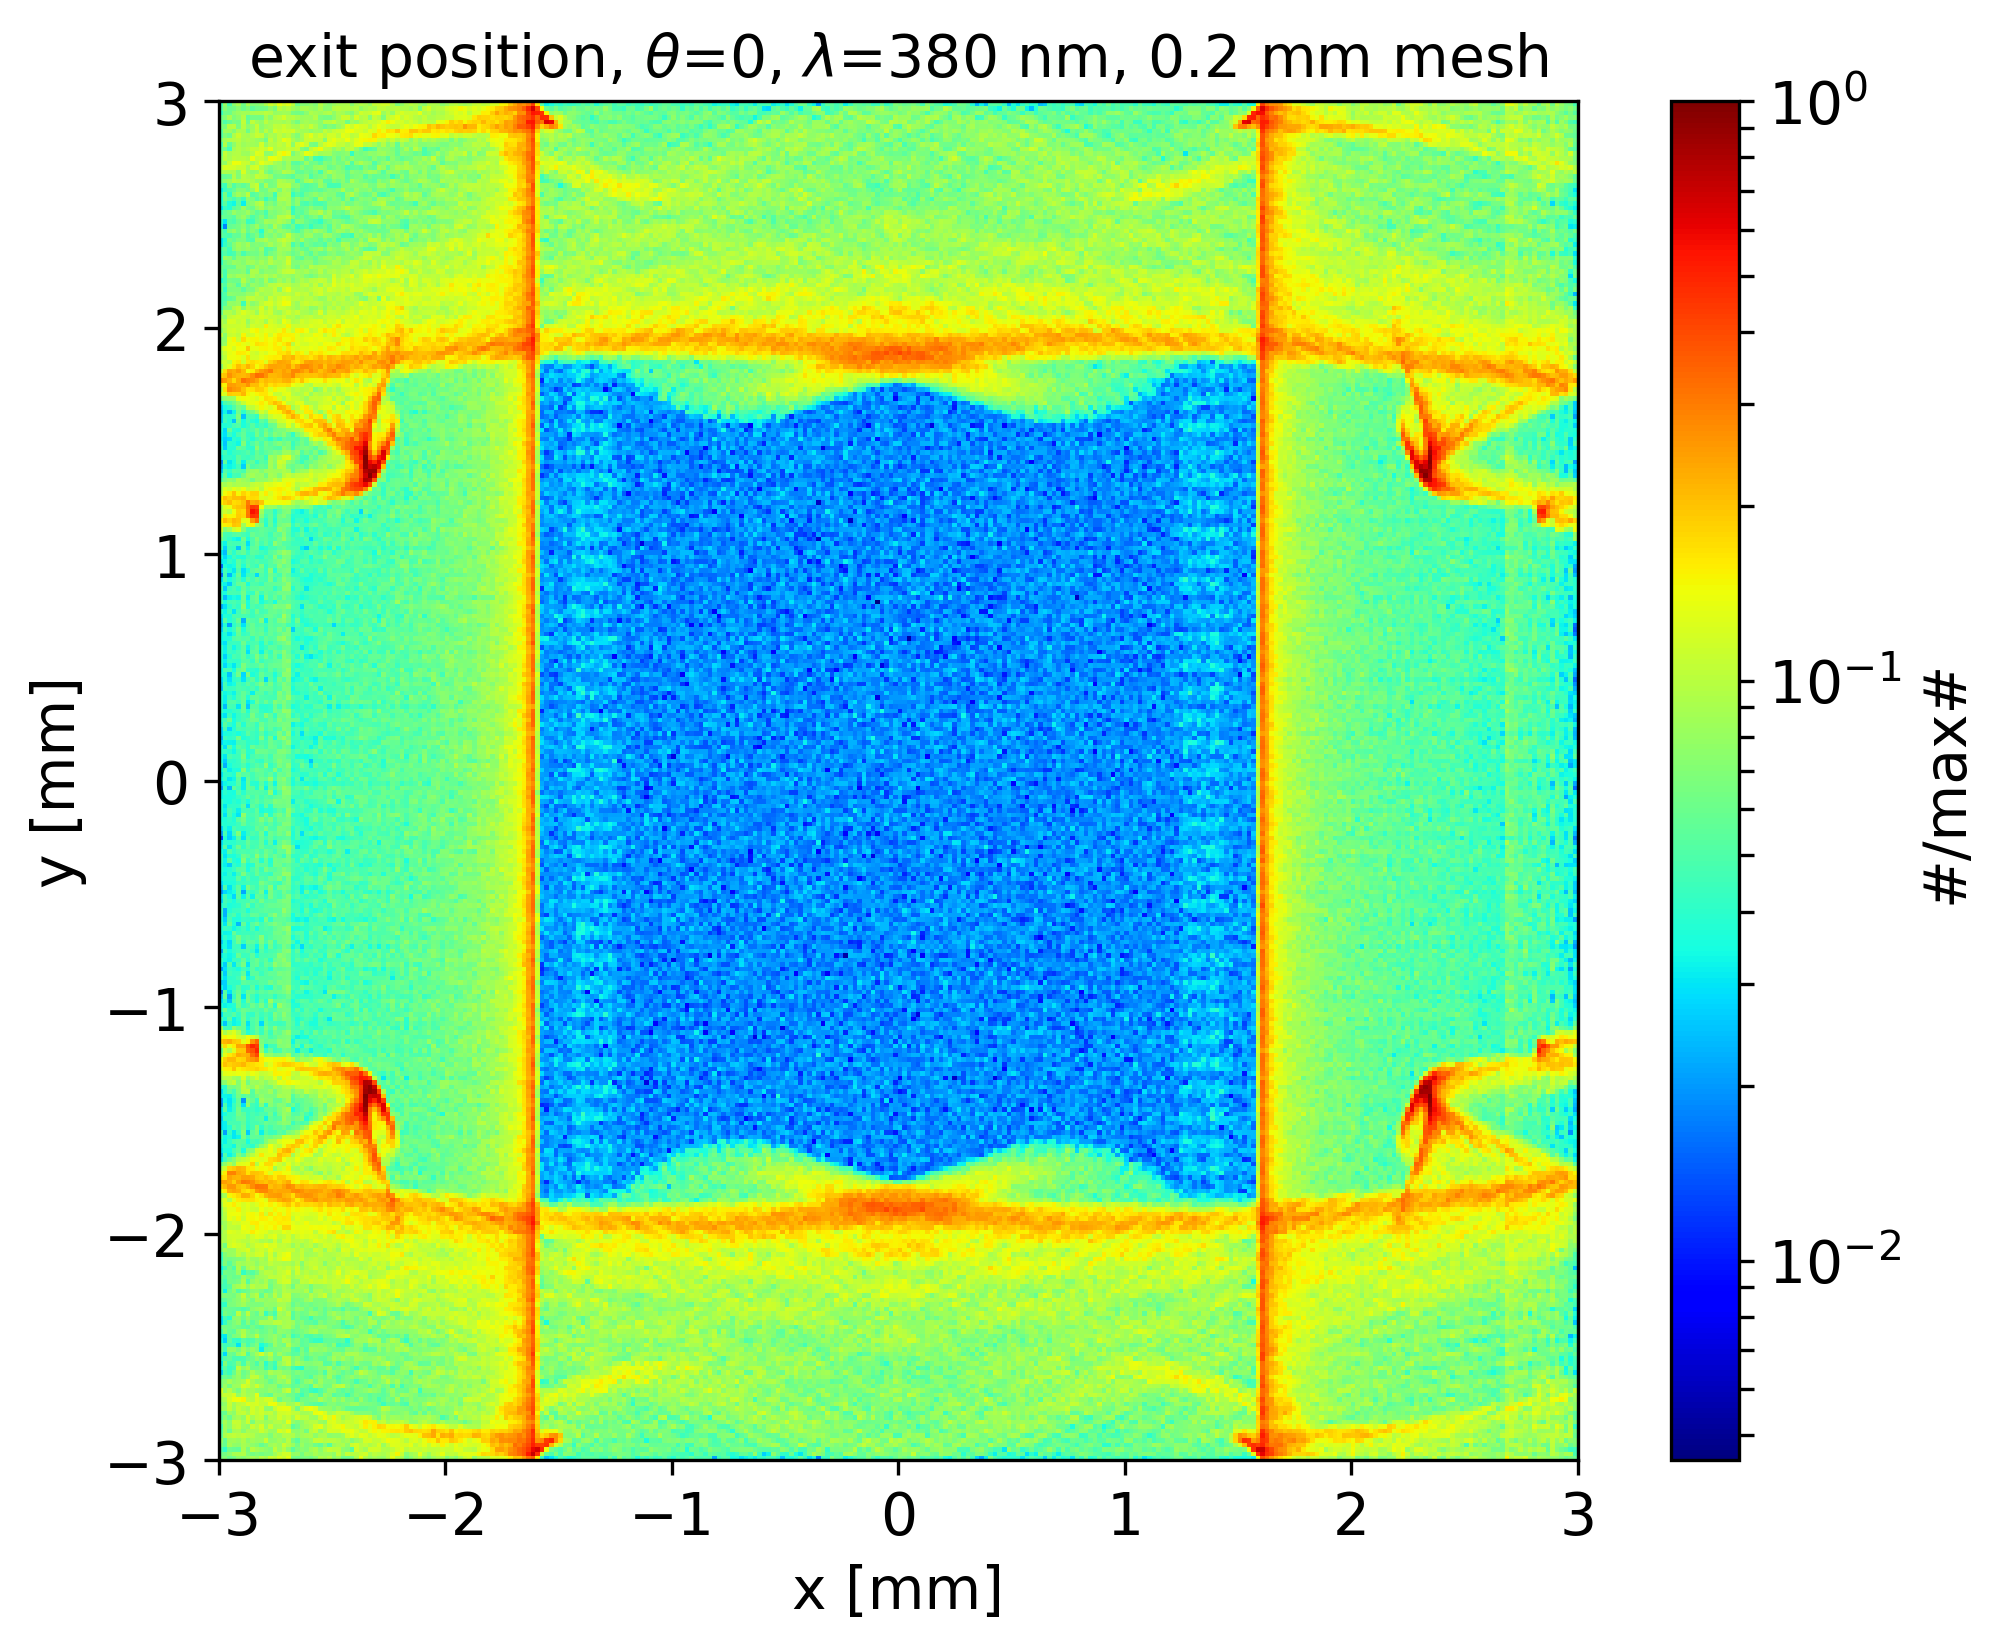
\includegraphics[width=\textwidth]{wico-theta0/hist_theta0_380nm-0.2mmMesh_log.png}
		\subcaption{$m=\SI{0.2}{\milli\meter}$.}
	\end{subfigure}
	\vfill
	\begin{subfigure}[t]{0.495\textwidth}
		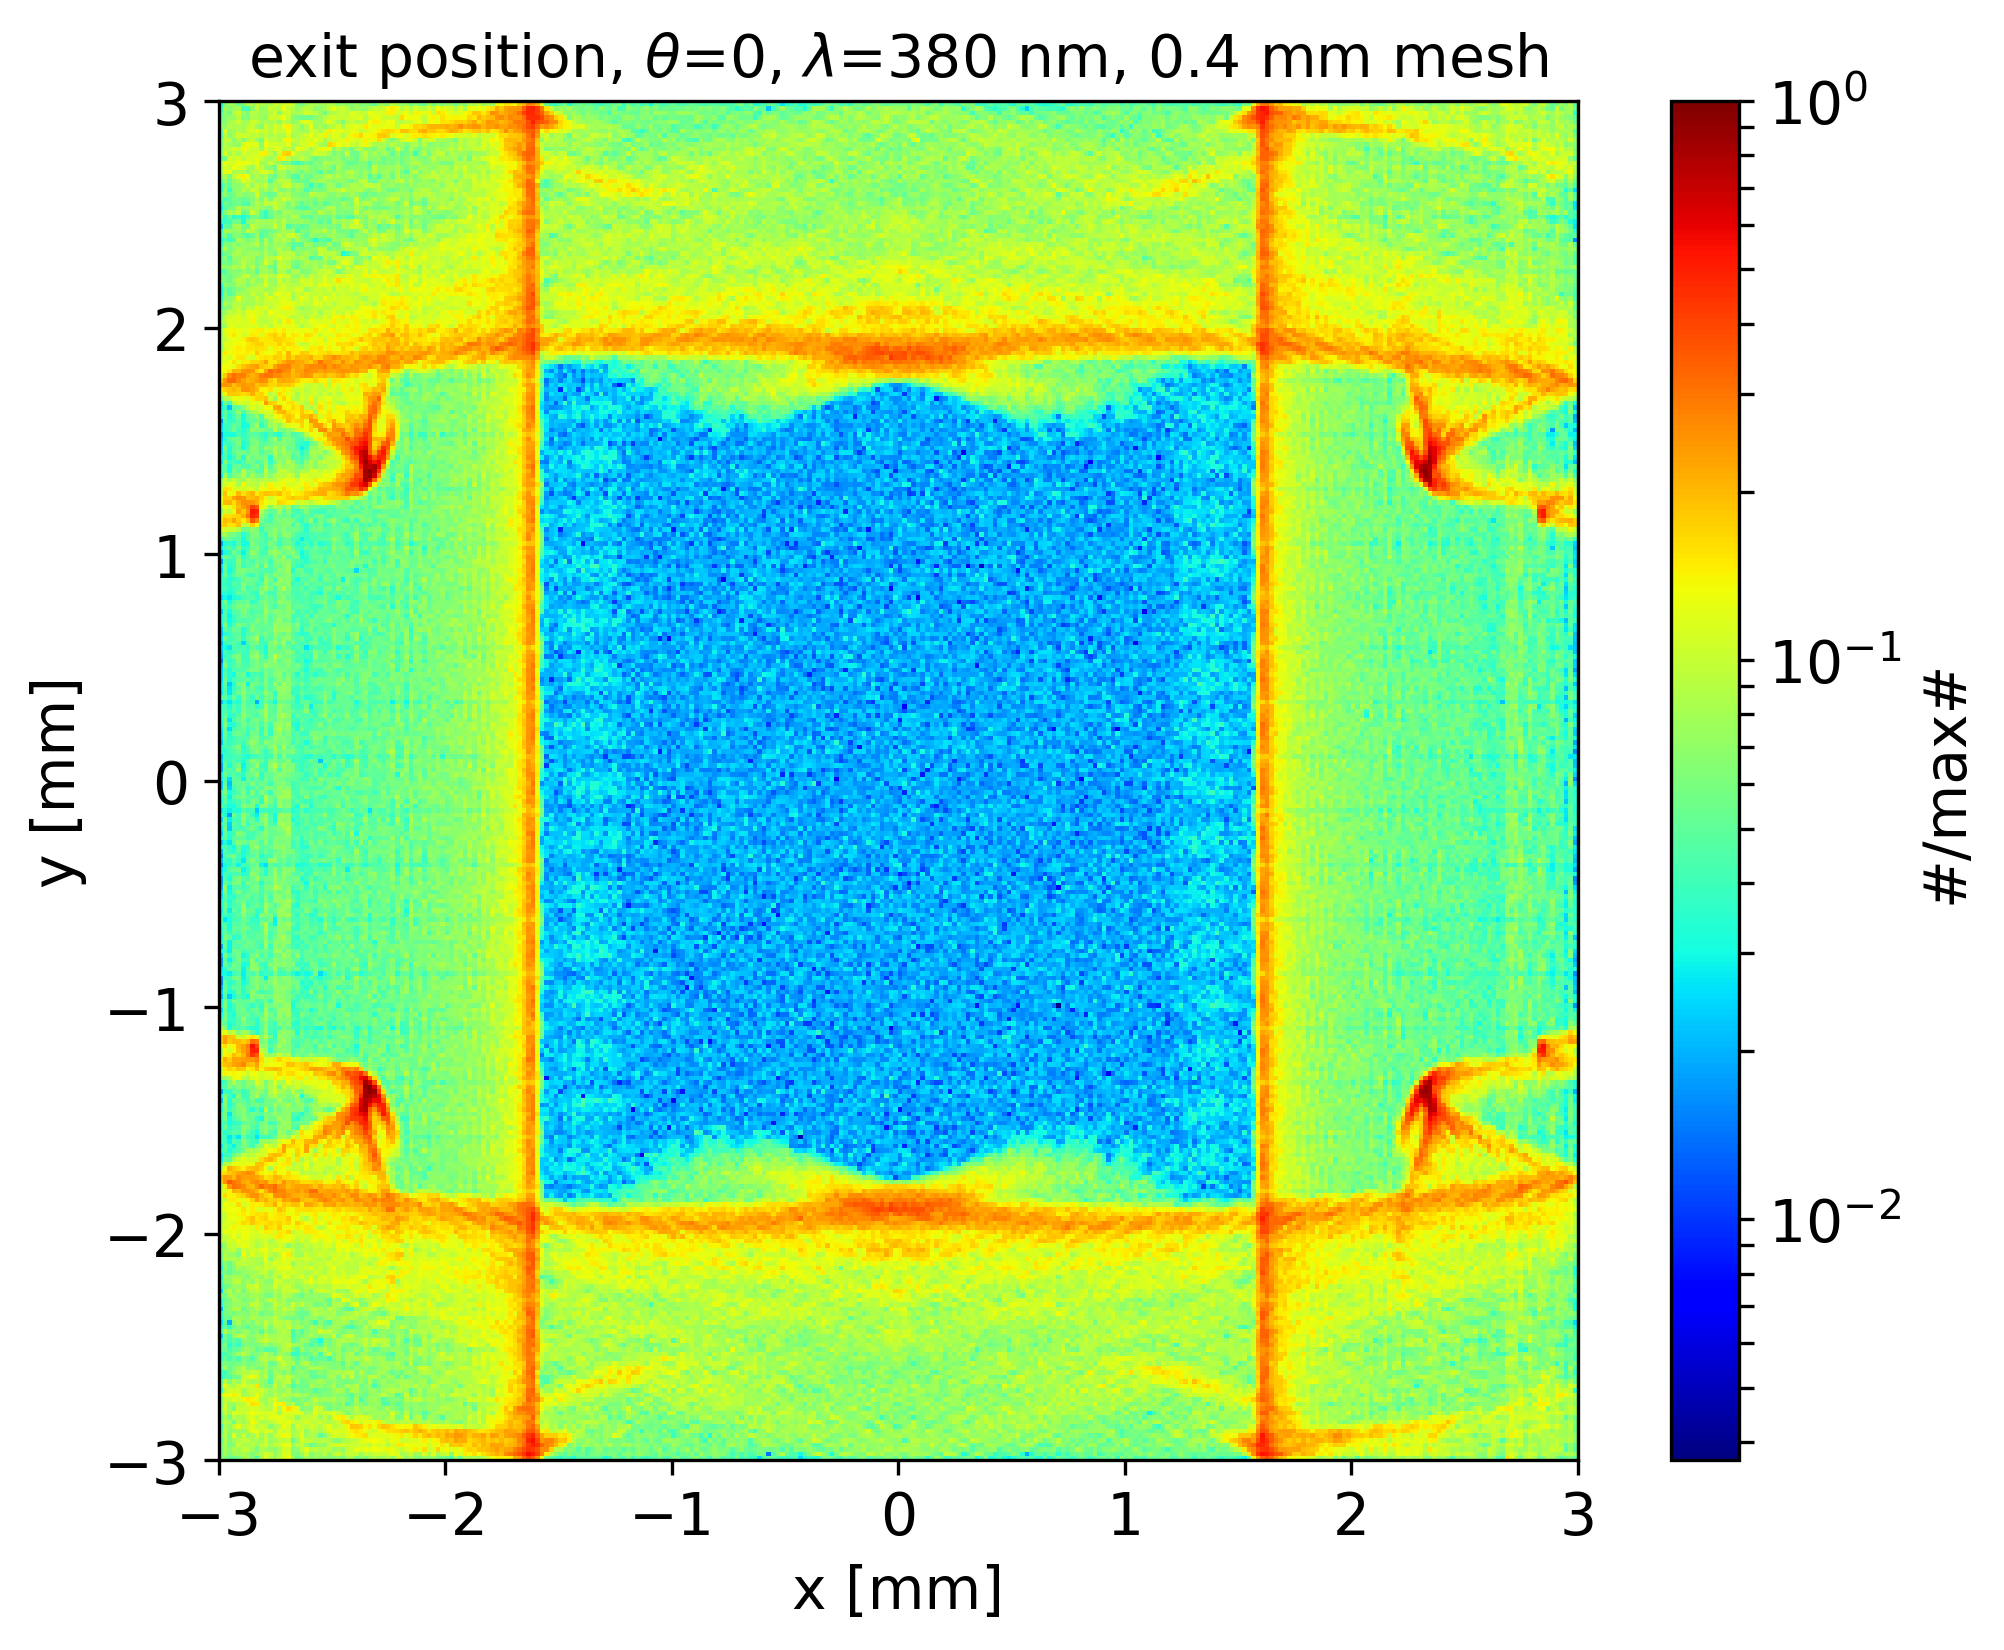
\includegraphics[width=\textwidth]{wico-theta0/hist_theta0_380nm-0.4mmMesh_log.png}
		\subcaption{$m=\SI{0.4}{\milli\meter}$.}
		\label{wico:theta0_image:m04}
	\end{subfigure}
	\hfill
	\begin{subfigure}[t]{0.495\textwidth}
		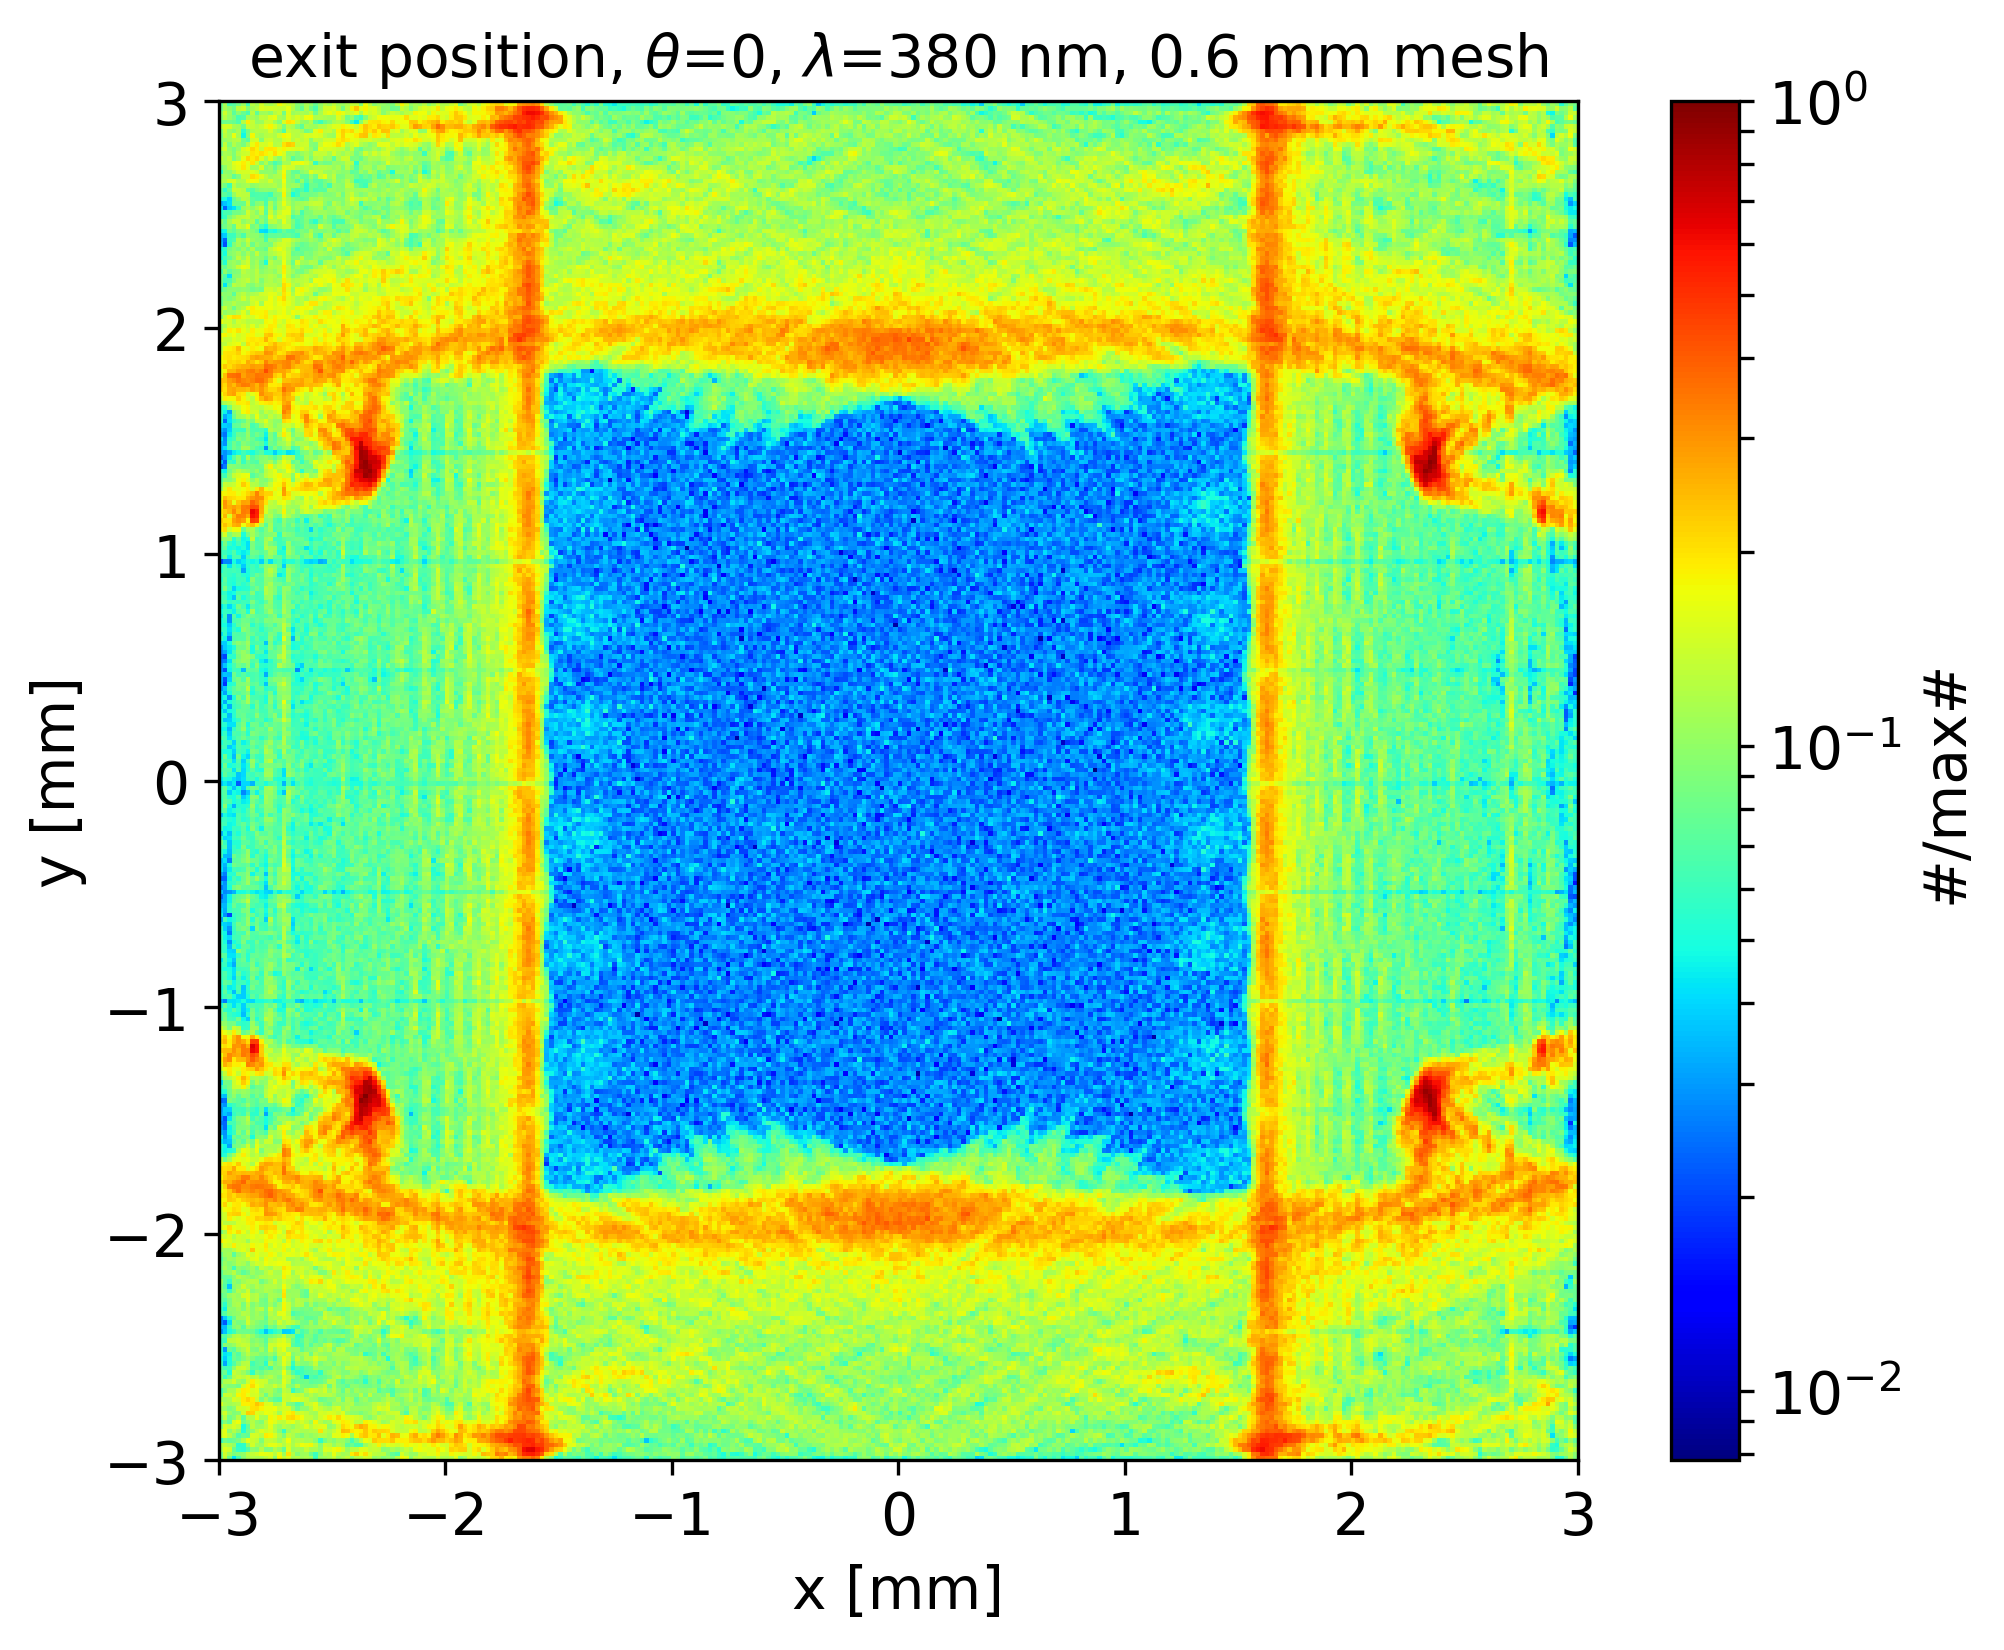
\includegraphics[width=\textwidth]{wico-theta0/hist_theta0_380nm-0.6mmMesh_log.png}
		\subcaption{$m=\SI{0.6}{\milli\meter}$.}
	\end{subfigure}
	\hfill
	\begin{subfigure}[t]{0.495\textwidth}
		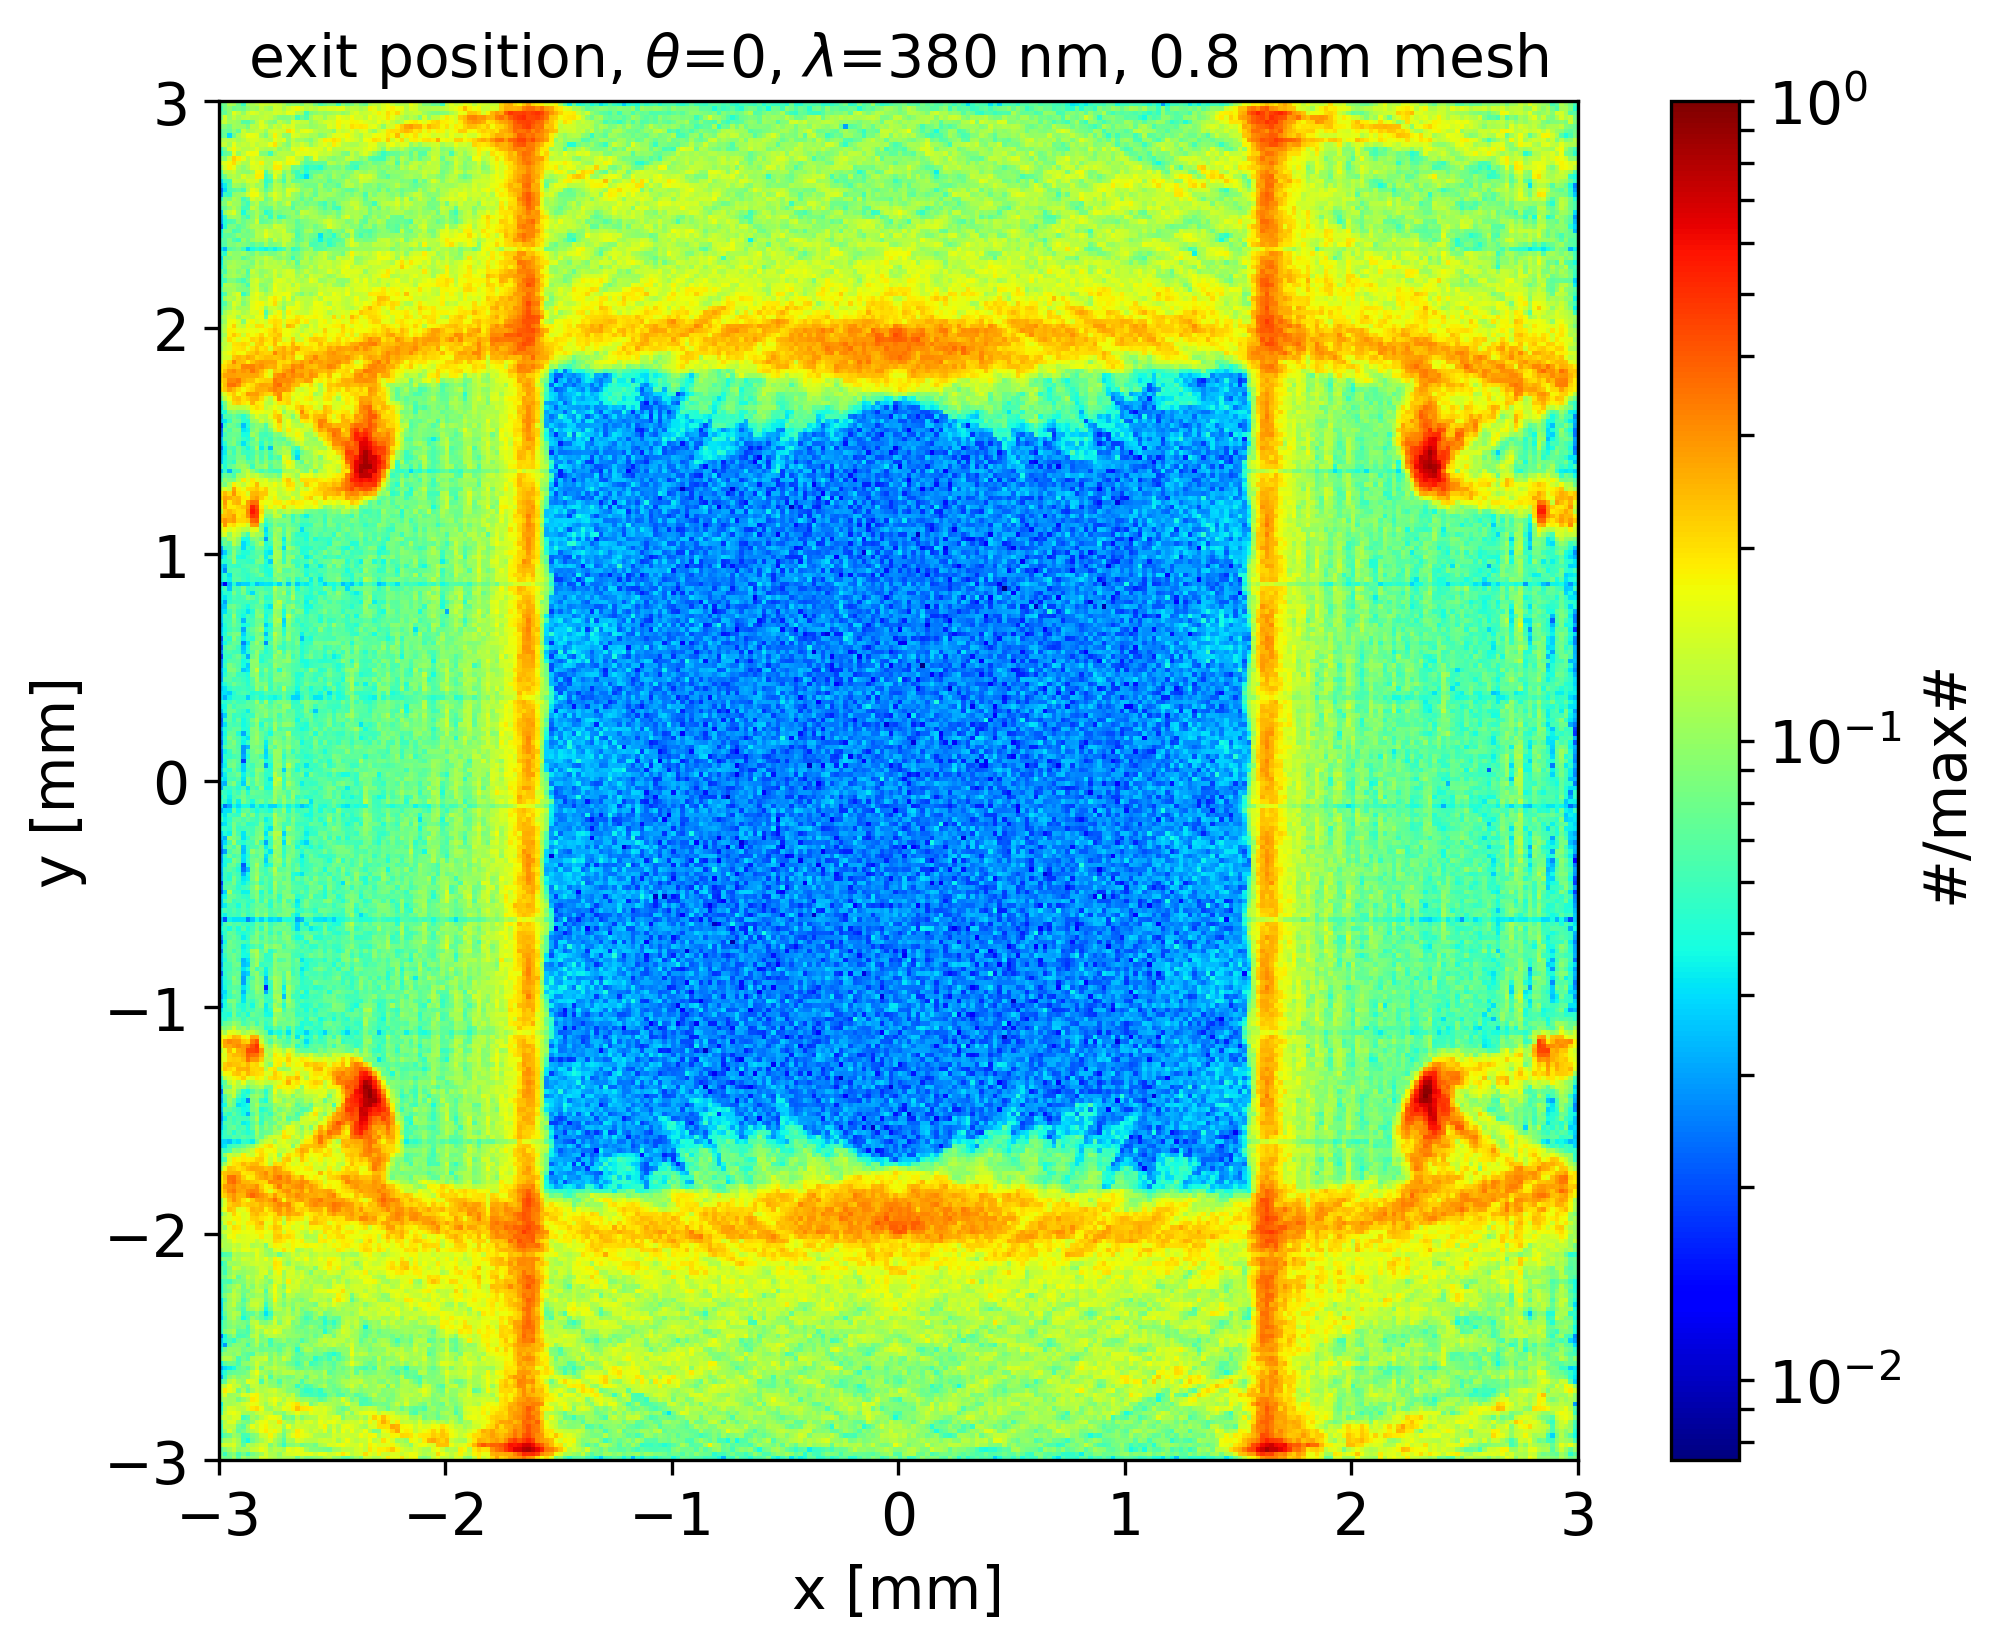
\includegraphics[width=\textwidth]{wico-theta0/hist_theta0_380nm-0.8mmMesh_log.png}
		\subcaption{$m=\SI{0.8}{\milli\meter}$.}
	\end{subfigure}
	\hfill
	\begin{minipage}[t]{0.495\textwidth}
		\vspace{-190pt}
		\caption[\enquote{Image} produced by the \iceact Winston cone]{\textbf{\enquote{Image} produced by the \iceact Winston cone.} The Winston cone is fully illuminated by vertical light ($\theta=\SI{0}{\degree}$) with $\lambda=\SI{380}{\nano\meter}$ and locations of arriving photons at the exit window are histogramized in a normalized logarithmic scale. This simulation is done with five different maximum edge lengths $m$ of the mesh. For $m\geq\SI{0.4}{\milli\meter}$, distinct artifacts are visible. $x$ and $y$ are the \geant coordinates as shown in figure~\ref{geant_coords}.}
	\end{minipage}
	\label{wico:theta0_image}
\end{figure}

In order to compare the meshed Winston cone with the exact CAD model, the \geant simulation is compared with the Zemax\footnote{Zemax is a commercial ray tracing tool for Microsoft Windows. It is commonly used for the analysis and optimization of optical systems.} simulation done in~\cite{iceact:camera}. Figure~\ref{wico:comparison_zemax} shows a quite high similarity.

\begin{figure}[H]
	\centering
	\saveimageheight[width=0.57\textwidth]{wico-theta0/hist_theta0_380nm-0.4mmMesh.png}
	\begin{subfigure}[t]{0.41\textwidth}
		\raiseimage[width=\textwidth]{WiCoTheta0_Zemax.png}
		\subcaption{Zemax simulation~\cite{iceact:camera}.}
	\end{subfigure}
	\hfill
	\begin{subfigure}[t]{0.57\textwidth}
		\usebox{\savedimage}
		\subcaption{\geant simulation with $m=\SI{0.4}{\milli\meter}$. This is the same data as shown in figure~\ref{wico:theta0_image:m04} but with linear scaling.}
	\end{subfigure}
	\caption[Comparison between \geant and Zemax simulation]{\textbf{Comparison between \geant and Zemax simulation.} For the main structure of the image by vertical illumination, \geant produces a quite similar image to the Zemax simulation done in~\cite{iceact:camera}.}
	\label{wico:comparison_zemax}
\end{figure}

In order to quantify the complexity of the meshed model, one can look at the file size for different mesh sizes. For the five investigated mesh sizes, this is done in table~\ref{wico:diskspace}.

\begin{table}[H]
	\centering
	\begin{tabular}{S[table-format=1.1]|S[table-format=5.0]|S[table-format=3.2]}
		\toprule
		\multicolumn{1}{c|}{mesh size $m$ [\si{\milli\meter}]} & \multicolumn{1}{c|}{size of meshed CAD file [\si{\kibi\byte}]} & \multicolumn{1}{c}{approx. loading time [\si{\second}]} \\
		\midrule
		0.1 & 18385 & 385\\
		0.2 &  4581 & 23.8\\
		0.4 &  2003 & 3.64\\
		0.6 &   520 & 0.35\\
		0.8 &   482 & 0.30\\
		\bottomrule
	\end{tabular}
	\caption[File size of Winston cone model for different mesh size]{\textbf{File size of Winston cone model for different mesh size.} Additionally, the approximate loading time of one Winston cone is given (on a single CPU core at \SI{1.4}{\giga\hertz}).}
	\label{wico:diskspace}
\end{table}

In summary, the mesh size $m=\SI{0.4}{\milli\meter}$ is chosen for the parameterization simulation since only slight artifacts are produced (cf. figure~\ref{wico:theta0_image:m04}). Additionally, it can reproduce the Zemax simulation quite well and with a file size of about \SI{2}{\mebi\byte}, the loading time is at a just reasonable time scale of a few seconds.

\subsection{\enquote{Ghost Image}}\label{sec:ghost_image}

At all interfaces, the photon has to pass, reflection and transmission occur. In the \iceact optics, mainly the transmission is desired. Nevertheless, reflections occur as well. To get a rough estimate, one can assume perpendicular incidence and evaluate equation~\eqref{eq:perp_interface_transmission} with $n(\lambda)=\num{1.5}$, $n_\text{air}=1$. The result is, that a photon is transmitted by $\approx\SI{96}{\percent}$ and reflected by $\approx\SI{4}{\percent}$. Usually, an incidental reflection results in \enquote{diffuse} scattering of the photons and decreases the imaging quality of the optical system. Besides this effect which results in a kind of \enquote{noisy} image, there is a very systematic beam path that ends up with a accumulation of scattered photons in a distinct direction -- the \textit{ghost image}. The reason for this effect is the glass plate in combination with the Fresnel lens. The imaging character of a lens translates an incident direction into a position on the focal plane. It can appear, that a photon is reflected at the Winston cone entrance window and thus gets back to the Fresnel lens. The Fresnel lens can now refract the photon in such a way that it gets to the back of glass plate namely with the same inclination angle as in the initial state, but now with the reversed traveling direction. A possible reflection on the glass plate results in a shift of the azimuth angle by \SI{180}{\degree}. By a trasmission through the Fresnel lens once again, the photon is now refracted to the focal plane with a azimuth shift of \SI{180}{\degree} as well. If now this photon gets finally through the cone and is detected by the SiPM, it causes the ghost image. To visualize this, figure~\ref{ghostimage_path} shows the ghost image effect at \enquote{leading order}, i.e. the most probable beam path.

\begin{figure}[H]
	\centering
	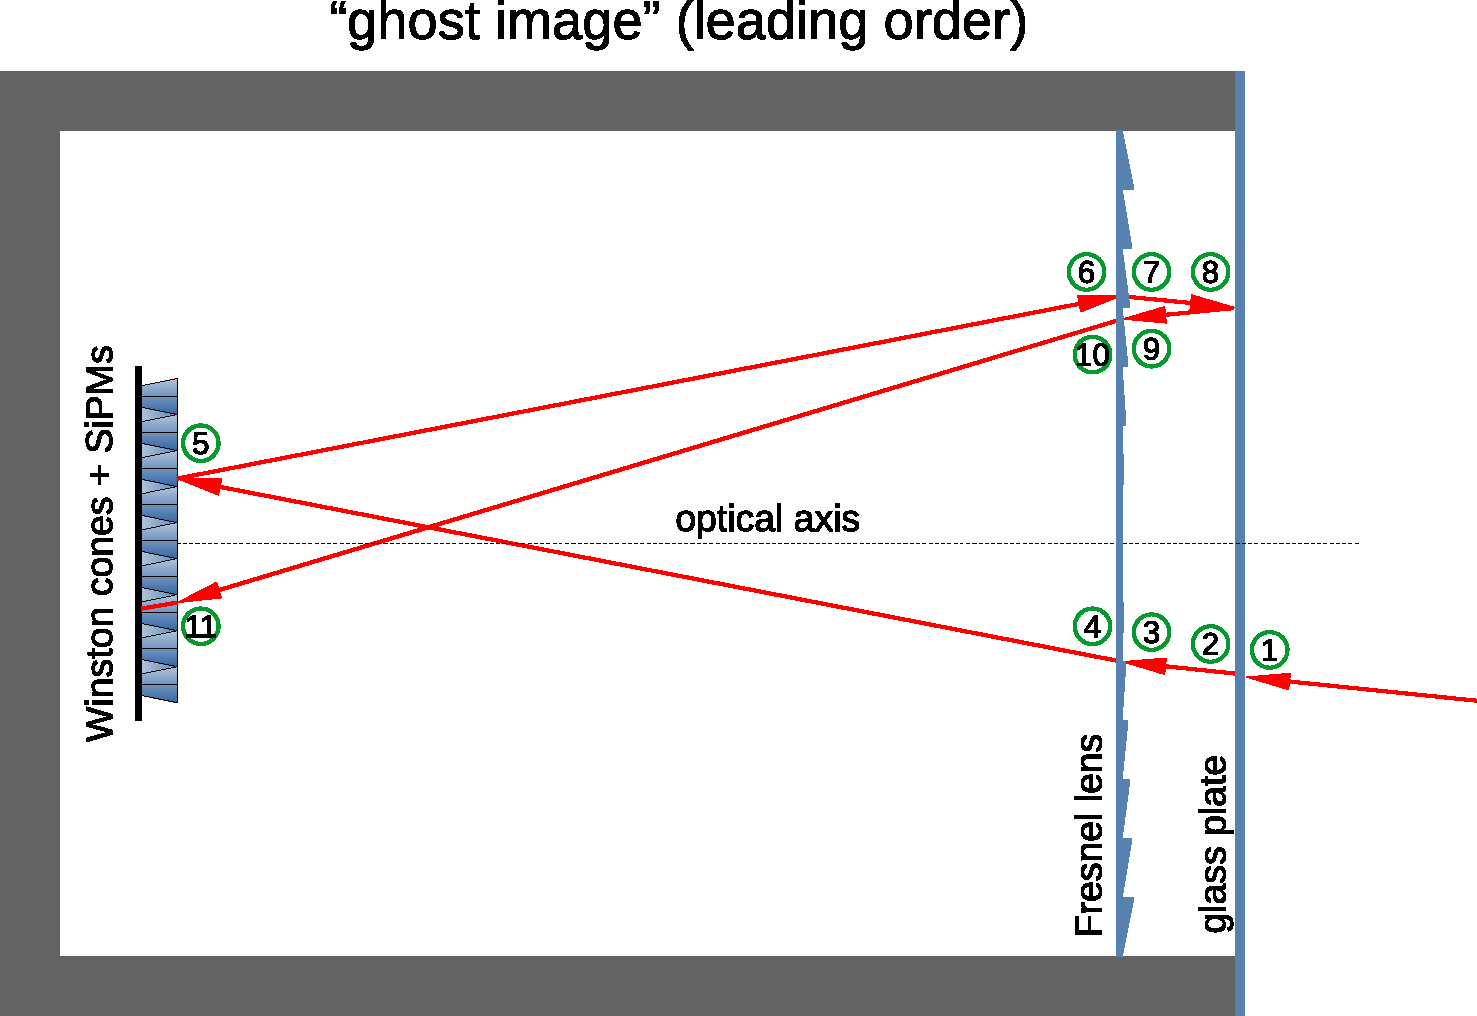
\includegraphics[width=0.7\textwidth]{GhostImage.pdf}
	\caption[Schematic sketch for the \enquote{ghost image} beam path]{\textbf{Schematic sketch for the \enquote{ghost image} beam path.} The encircled numbers mark the order of interface interactions. At 1, 2, 3, 4, 6, 7, 9, 10, and 11, transmission is required whereas at 5 and 8, the photon needs to be reflected in order to produce the ghost image. At 8, the azimuth shift of \SI{180}{\degree} takes place.}
	\label{ghostimage_path}
\end{figure}

With the approximated transmission and reflection coefficient one can estimate the suppression factor. The ghost image occurs if a photon undergoes two reflections and four transmissions more than a \enquote{normal} photon that is detected in the right SiPM. Thus, one gets a suppression factor of
\begin{align}
	(\SI{4}{\percent})^2 \cdot (\SI{96}{\percent})^4 \sim \SI{0.1}{\percent}\,.
\end{align}
One obtains, that the ghost image is a per-mill effect, i.e. for an image where \num{1000} photons are detected, one would expect one ghost image photon. The detection efficiency maps in figure~\label{deteff:offaxis_px} show some examples for the ghost image effect. It causes a suppressed mirror image of the core efficiency region.

\section{Parameterization Simulation}

The parameterization has the goal to give the detection efficiency of each pixel for a photon with given wavelength $\lambda$ and direction $(\theta,\phi)$. Therefore, a simulation has to be done for a wavelength range $[\lambda_\text{min}, \lambda_\text{max}]$ and a direction range -- given by a maximum inclination angle $\theta_\text{max}$ -- in which \iceact is capable of detecting Cherenkov photons. Firstly, the \geant coordinate system is introduced in figure~\ref{geant_coords}.\\

\begin{figure}[H]
	\centering
	\saveimageheight[width=0.49\textwidth]{GeantCoords.pdf}
	\begin{subfigure}[t]{0.49\textwidth}
		\raiseimage[width=\textwidth]{CameraPixels.pdf}
		\subcaption{Top view of the \iceact camera with pixel numbering and coordinate system. The $z$-axis comes out of the drawing plane.}
	\end{subfigure}
	\hfill
	\begin{subfigure}[t]{0.49\textwidth}
		\usebox{\savedimage}
		\subcaption{Coordinate system for the \iceact telescope. The tube is sketched as a the blue cylinder. The coordinate origin is set as the center of the focal plane on the Winston cones' entrance windows. An exemplary incoming photon drawn as red line impinges on the glass plate under a zenith angle $\theta$ and an azimuth angle $\phi$.}
	\end{subfigure}
	\caption[Coordinate system used in \geant and for the simulation]{\textbf{Coordinate system used in \geant and for the simulation.} }
	\label{geant_coords}
\end{figure}

The wavelength range is mainly limited by the material properties and the photon detection efficiency of the SiPMs (cf. figures~\ref{iceact:model:material:transmission} and \ref{sipm:pde}). The layout of the optical system determines the maximum inclination angle. In figure~\ref{iceact:camera:layout} a maximum inclination angle of $\approx\SI{6.8}{\degree}$ is calculated. For this parameterization, a larger angle of $\theta_\text{max}=\SI{10}{\degree}$ is chosen in order to account for UV photons near $\lambda_\text{min}$  which are refracted more strongly and thus can be detected under higher zenith angles. Both -- i.e. wavelengths and directions -- are simulated uniformly distributed. For $\lambda$ and $\phi$ this can be done without problems. For the zenith angle $\theta$ one has to consider the curvilinear character of the spherical coordinate system, which causes a variable phase space depending on $\theta$. By taking the cosine of the zenith angle, this effect is compensated. Thus, the simulation is done uniformly in $\cos{\theta}$. Additionally, the focal plane shift (cf. section~\ref{sec:focalplaneshift}) and the reasonable mesh size (cf. section~\ref{sec:wico_meshing}) is applied. In total, \num{15e9} particles are simulated. Table~\ref{paramsim:params} gives a summary of the simulation parameters.

\begin{table}[H]
	\centering
	\begin{tabular}{r|c|l}
		\toprule
		description 				   & symbol               & value\\
		\midrule
		minimum simulated wavelength   & $\lambda_\text{min}$ & \SI{272}{\nano\meter}\\
		maximum simulated wavelength   & $\lambda_\text{max}$ & \SI{900}{\nano\meter}\\
		maximum simulated zenith angle & $\theta_\text{max}$  & \SI{10}{\degree}\\
		mesh size (maximum edge length)& $m$				  & \SI{0.4}{\milli\meter}\\
		focal plan shift 			   & $\Delta z$			  & \SI{1.25}{\milli\meter}\\
		total simulated particles      & $N_\text{sim}$		  & \num{15e9}\\
		\bottomrule
	\end{tabular}
	\caption[Parameters chosen for the parameterization simulation]{\textbf{Parameters chosen for the parameterization simulation.} Wavelengths are simulated uniformly in the interval $[\lambda_\text{min}, \lambda_\text{max}]$. The direction are simulated uniformly in azimuth $\phi$ and cosine of the zenith angle $\cos{\theta}$. The reasonable mesh size determined in section~\ref{sec:wico_meshing} and the focal plane shift discussed in section~\ref{sec:focalplaneshift} is applied.}
	\label{paramsim:params}
\end{table}

\todo{ebene welle, volle ausleuchtung der glasplatte}